\documentclass[10pt,a4paper]{extreport}

\usepackage{amsmath}
\usepackage{enotez}
\setenotez{list-name=Notas,totoc=chapter}
\renewcommand\theendnote{\underline{\arabic{endnote}}}
\usepackage{titling}
\usepackage{float}
\usepackage{placeins}
\usepackage{esint}
\newcommand{\aspas}[1]{``#1''}
\usepackage{amsfonts}
\usepackage[tight,normalsize]{subfigure}
\usepackage{amssymb}
\usepackage[font=large]{caption}
\usepackage{wrapfig}
\usepackage{nicefrac}
\usepackage{mathtools}
\usepackage[per-mode=symbol]{siunitx}
\usepackage[ddmmyyyy]{datetime}
\usepackage[margin=1.0in]{geometry}
\usepackage{indentfirst}
\usepackage{courier}
\usepackage{graphicx}
\usepackage{xurl}
\usepackage{hyperref}
\usepackage{afterpage}
\usepackage{listings}
\usepackage{lipsum}
\usepackage[table,xcdraw]{xcolor}
\usepackage{pgfplots}
\pgfplotsset{compat=1.15}
\usepackage{mathrsfs}
\usepackage{tikz}
\usetikzlibrary{arrows}
\usepackage{csquotes}
\usepackage[brazil]{babel}
\usepackage[style=abnt]{biblatex}
\setlength\bibitemsep{\baselineskip}
\renewcommand*{\bibfont}{\normalfont}
\addbibresource{referencias.bib}
\usepackage{titlesec}
\usepackage[acronym]{glossaries}

\renewcommand{\figurename}{Figura}
\renewcommand{\tablename}{Tabela}
\renewcommand{\j}{\ensuremath{j}}
\renewcommand{\ang}[1]{\ensuremath{\num{#1}^\circ}}
\newcommand{\eval}[2]{\left.#1\right|_{#2}}
\newcommand{\real}[1]{\Re\left\{#1\right\}}
\newcommand{\imag}[1]{\Im\left\{#1\right\}}
\newcommand{\op}[1]{\operatorname{#1}}
\newcommand{\pd}[3]{\frac{\partial^{#3} #1}{{\partial#2}^{#3}}}
\newcommand{\deriv}[3]{\frac{d^{#3} #1}{{d#2}^{#3}}}
\newcommand{\abs}[1]{\left\vert#1\right\vert}
\newcommand{\swr}{\operatorname{SWR}}
\newcommand{\ibv}{\hat{\mathrm{i}}}
\newcommand{\jbv}{\hat{\mathrm{j}}}
\newcommand{\kbv}{\hat{\mathrm{k}}}
\newcommand{\sen}{\operatorname{sen}}
\newcommand{\senh}{\operatorname{senh}}
\newcommand{\tg}{\operatorname{tg}}
\newcommand{\tgh}{\operatorname{tgh}}
\newcommand{\R}{\mathbb{R}}
\newcommand{\C}{\mathbb{C}}
\newcommand{\N}{\mathbb{N}}
\newcommand{\Z}{\mathbb{Z}}
\newcommand{\p}{\mathcal{P}}
\newcommand{\lt}[1]{\mathcal{L}\left\{#1\right\}}
\newcommand{\ilt}[1]{\mathcal{L}^{-1}\left\{#1\right\}}
\newcommand{\?}{\stackrel{?}{=}}
\newcommand{\pol}[2]{\complexnum{#1}\angle\ang{#2}}
\newcommand{\sir}[2]{\complexnum{#1}\,\si[per-mode=reciprocal]{#2}}
\newcommand{\sif}[2]{\complexnum{#1}\,\si[per-mode=fraction]{#2}}
\newcommand{\sis}[2]{\complexnum{#1}\,\si[per-mode=symbol]{#2}}
\newcommand{\sip}[3]{\left(\pol{#1}{#2}\right)\,\si[per-mode=symbol]{#3}}
\newcommand{\sic}[3]{\left(\num{#1}\num[retain-explicit-plus]{#2}\j\right)\si[per-mode=symbol]{#3}}
\newcommand{\siv}[1]{\left[\si{#1}\right]}
\sisetup{output-decimal-marker = {,}}
\sisetup{output-complex-root=\j}
\sisetup{input-digits = 0123456789\pi}

\newcommand{\mysize}{0.69}

\DeclareSIUnit{\dbm}{dBm}
\DeclareSIUnit{\dbw}{dBW}
\DeclareSIUnit{\dbi}{dBi}
\DeclareSIUnit{\voltrms}{\ensuremath{\si{\volt}_{\text{rms}}}}
\DeclareSIUnit{\ampererms}{\ensuremath{\si{\ampere}_{\text{rms}}}}
\DeclareSIUnit{\va}{\si{VA}}
\DeclareSIUnit{\var}{\si{VAr}}

\hypersetup{
    colorlinks,
    linkcolor={black},
    citecolor={black},
    urlcolor={blue!80!black}
}

\makeatletter
\renewcommand*\env@matrix[1][*\c@MaxMatrixCols c]{%
	\hskip -\arraycolsep
	\let\@ifnextchar\new@ifnextchar
	\array{#1}}
\makeatother

\DeclareInstance{enotez-list}{custom}{paragraph}
{
heading=\chapter*{#1},
notes-sep=\baselineskip,
format=\normalfont,
number=\textsuperscript{#1}
}

\usepackage{afterpage}
\newcommand\myemptypage{
    \null
    \thispagestyle{empty}
    \addtocounter{page}{-1}
    \newpage
    }

\AtBeginDocument{
\addtolength{\abovedisplayskip}{-1ex}
\addtolength{\abovedisplayshortskip}{-1ex}
\addtolength{\belowdisplayskip}{1ex}
\addtolength{\belowdisplayshortskip}{1ex}
}

\makeglossaries
\newacronym{mosfet}{MOSFET}{\textit{Metal-Oxide-Semiconductor Field Effect Transistor}}
\newacronym{scm}{SCM}{\textit{Self Cascode} \acrshort{mosfet}}
\newacronym{sbcs}{SBCS}{\textit{Self-Biased Current Source}}
\newacronym{acm}{ACM}{\textit{Advanced Compact} \acrshort{mosfet}}
\newacronym{uicm}{UICM}{\textit{Unified Current-Control Model}}
\newacronym{lci}{LCI}{Laboratório de Circuitos Integrados}
\newacronym{tsmc}{TSMC}{\textit{Taiwan Semiconductor Manufacturing Company}}
\newacronym{cmos}{CMOS}{\textit{Complementary Metal–Oxide–Semiconductor}}
\newacronym{vfcm}{VFCM}{\textit{Voltage-Follower Current Mirror}}
\newacronym{pibic}{PIBIC}{Programa Institucional de Bolsas de Iniciação Cientifica}

%\begin{wrapfigure}{l}{0.4\textwidth}
%    \begin{center}
%        \includegraphics[width=0.384\textwidth]{Imagens/figura}
%    \end{center}
%    \caption{caption}
%    \label{label}
%\end{wrapfigure}

%\begin{figure}[htp!]
%    \caption{Caption}
%    \label{fig:label}
%    \includegraphics[width=\linewidth]{imagens/imagem.png}
%    \centering
%\end{figure}

\begin{document}
\begingroup
\renewcommand{\thepage}{0}
\begin{titlepage}
    \begin{center}
        \vspace*{1cm}
        \Huge
        \textbf{PROJETO DE FONTE DE BAIXÍSSIMA CORRENTE AUTO-POLARIZADA PARA CIRCUITOS INTEGRADOS \acrshort{cmos} DE BAIXO CONSUMO}
             
        \vspace{1.5cm}

        Relatório Final de \\
        pesquisa de Iniciação Científica\\
        \acrshort{pibic} 2021/2022\\
 
        \vfill
        \Large
        \textbf{Aluno: Victor Sabiá Pereira Carpes}\\
        \textbf{Orientador: Prof. Márcio Cherem Schneider, Dr.}
        \vspace{0.8cm}

        Departamento de Engenharia Elétrica e Eletrônica\\
        Curso de Graduação em Engenharia Eletrônica\\
        Universidade Federal de Santa Catarina\\
        Brasil\\
        
             
    \end{center}
\end{titlepage}
\endgroup
\myemptypage
\Large

\setcounter{lofdepth}{2}
\tableofcontents

\chapter*{Resumo}
\label{ch:resumo}
\addcontentsline{toc}{chapter}{\nameref{ch:resumo}}

Este trabalho apresenta os estudos realizados ao longo dos anos de 2021 e 2022 no \acrfull{lci} no projeto de uma fonte de corrente auto-polarizada baseada na estrutura \acrfull{scm}. A caracterização do \acrshort{scm} é feita através do modelo \acrfull{acm} desenvolvido por \cite{acm:book}, a partir da qual a fonte de corrente é projetada. O circuito final é baseado na topologia apresentada por \cite{sbcs} e foi implementado em simulação na tecnologia $\sis{180}{\nano\meter}$ da \acrshort{tsmc}. Apresenta, para uma tensão de saída fixa em $\sis{1.8}{\volt}$, uma corrente de saída $\sis{1.37}{\pico\ampere}$, um consumo máximo de $\sis{133}{\pico\watt}$ e uma regulação de linha média indo de $\sis{2.96}{\percent\per\volt}$ até $\sis{3.77}{\percent\per\volt}$ para diferentes tensões de saída. A sua sensibilidade média à temperatura na faixa de $\sis{0}{\celsius}$ até $\sis{100}{\celsius}$ é de $\sis{1.75}{\percent\per\celsius}$ e na faixa de $\sis{0}{\celsius}$ até $\sis{60}{\celsius}$ é de $\sis{1.01}{\percent\per\celsius}$.
\vspace{2cm}

\textbf{Palavas Chave:} \acrshort{cmos}, \acrshort{mosfet}, \acrshort{acm}, \textit{Low Power}, Fonte de Corrente, Design Analógico, Circuitos Integrados.

\newpage
\addcontentsline{toc}{chapter}{\listfigurename}
\listoffigures
\newpage
\addcontentsline{toc}{chapter}{Lista de Siglas e Acrônimos}
\printglossary[type=\acronymtype, title=Lista de Siglas e Acrônimos]


\newpage
Os códigos utilizados para as extrações de parâmetros, dimensionamento de componentes, geração de gráficos e elaboração deste próprio documento podem ser encontrados livremente no seguinte endereço:

\url{https://github.com/victorscarpes/relatorio_ic_lci}

\newpage

\setcounter{chapter}{0}
\chapter{Introdução}

Quando se trata de circuitos integrados, as células mais fundamentais são os espelhos e fontes de corrente, sendo eles responsáveis pela polarização dos outros blocos do circuito. Com avanços na miniaturização dos circuitos, cada vez mais as fontes de baixa corrente se mostram importantes. Nesta escala, uma boa regulação de linha e sensibilidade à temperatura se tornam muito complicadas, sendo necessário utilizar muita área e/ou transistores de dimensões muito extremas.

\section{Objetivo}

\begin{wrapfigure}[12]{r}{0.4\textwidth}
    \centering
    \vspace{-0.4cm}
    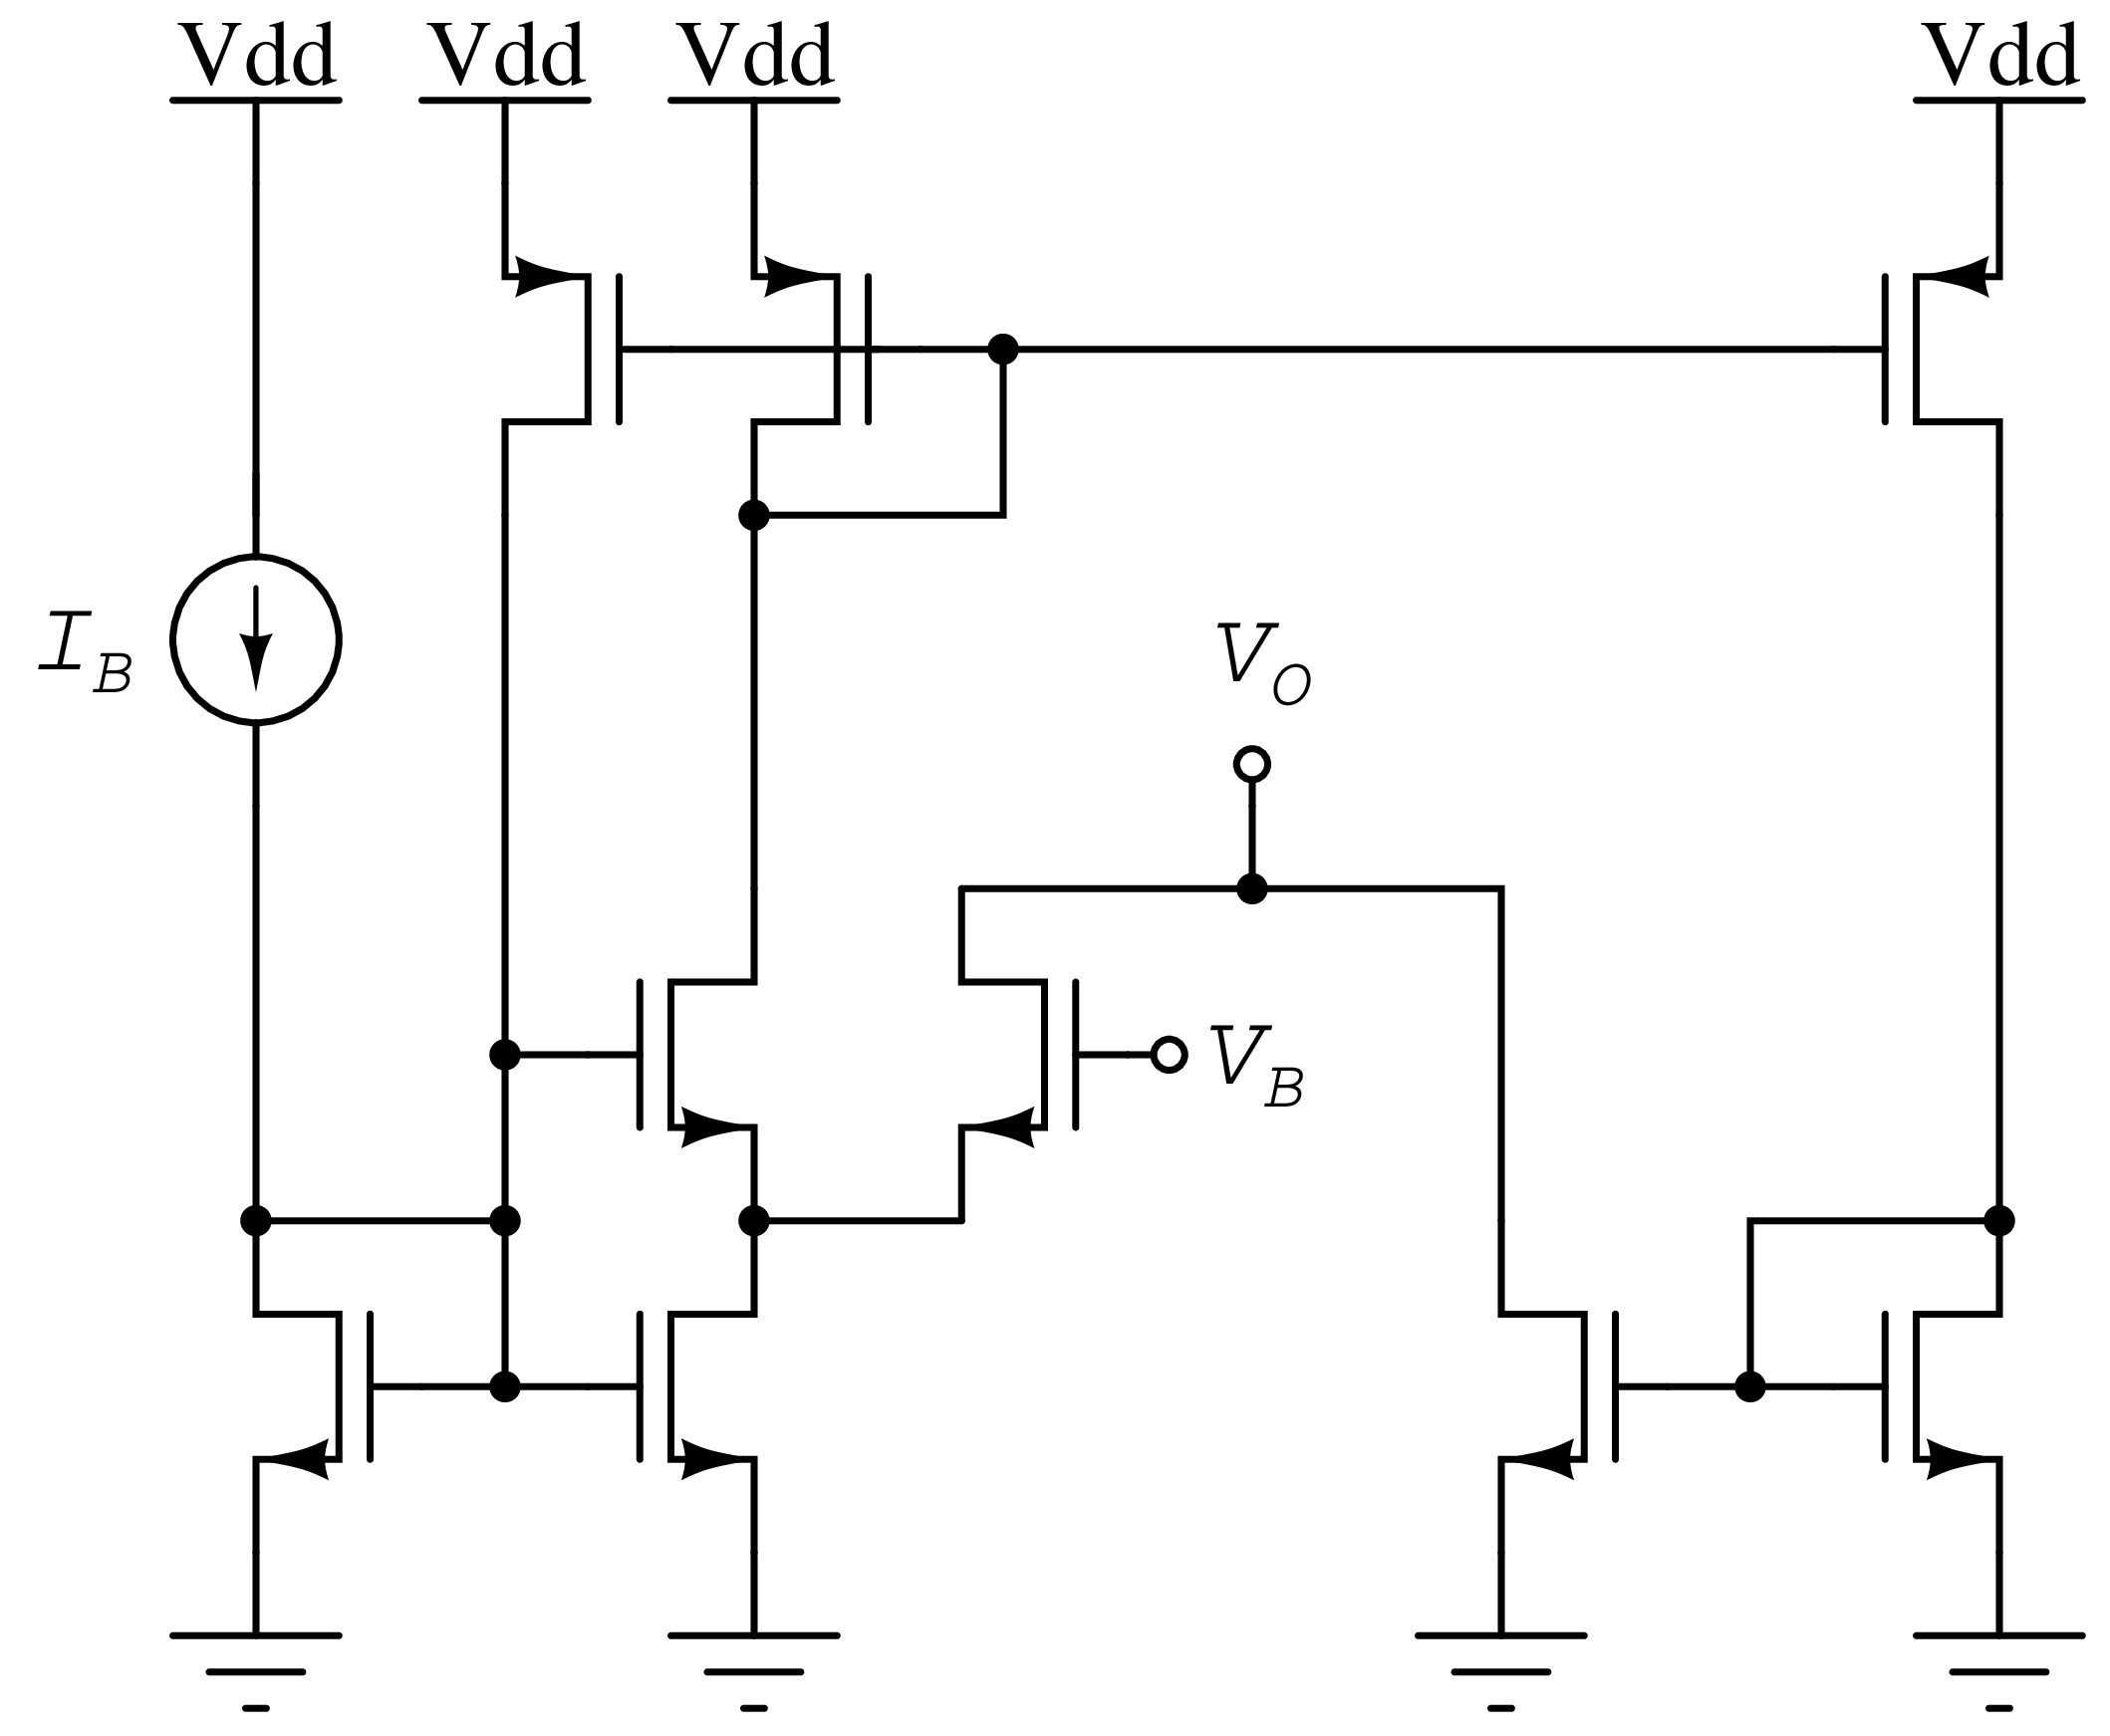
\includegraphics[width=0.4\textwidth]{Imagens/original_source.jpg}
    \caption{Diagrama da estrutura originalmente proposta pelo orientador.}
    \label{fig:original_source}
\end{wrapfigure}

Originalmente, o objetivo deste trabalho seria o desenvolvimento de uma fonte de corrente utilizando a estrutura apresentada na figura \ref{fig:original_source}, mas no meio do período da iniciação científica, o orientador decidiu por mudar a topologia. Após a mudança, o novo objetivo passou a ser a exploração de uma topologia de \acrfull{sbcs} de \cite{sbcs} para o projeto de uma fonte que opere nas proximidades de $\sis{1}{\pico\ampere}$.

Simulações para caracterização da regulação de linha e sensibilidade térmica serão apresentadas através do simulador Virtuoso da Cadence na tecnologia de $\sis{180}{\nano\meter}$ da \acrfull{tsmc}.

\chapter{Material e Métodos}
\section{Análise da estrutura \acrshort{scm}}

Nesta seção, a estrutura \acrshort{scm} da figura \ref{fig:scm_circuit} será analisada através do modelo de \cite{acm:book}. A dedução vai seguir um raciocínio similar ao apresentado em \cite{sbcs}.

\begin{wrapfigure}[15]{l}{0.35\textwidth}
    \centering
    \vspace{-0.4cm}
    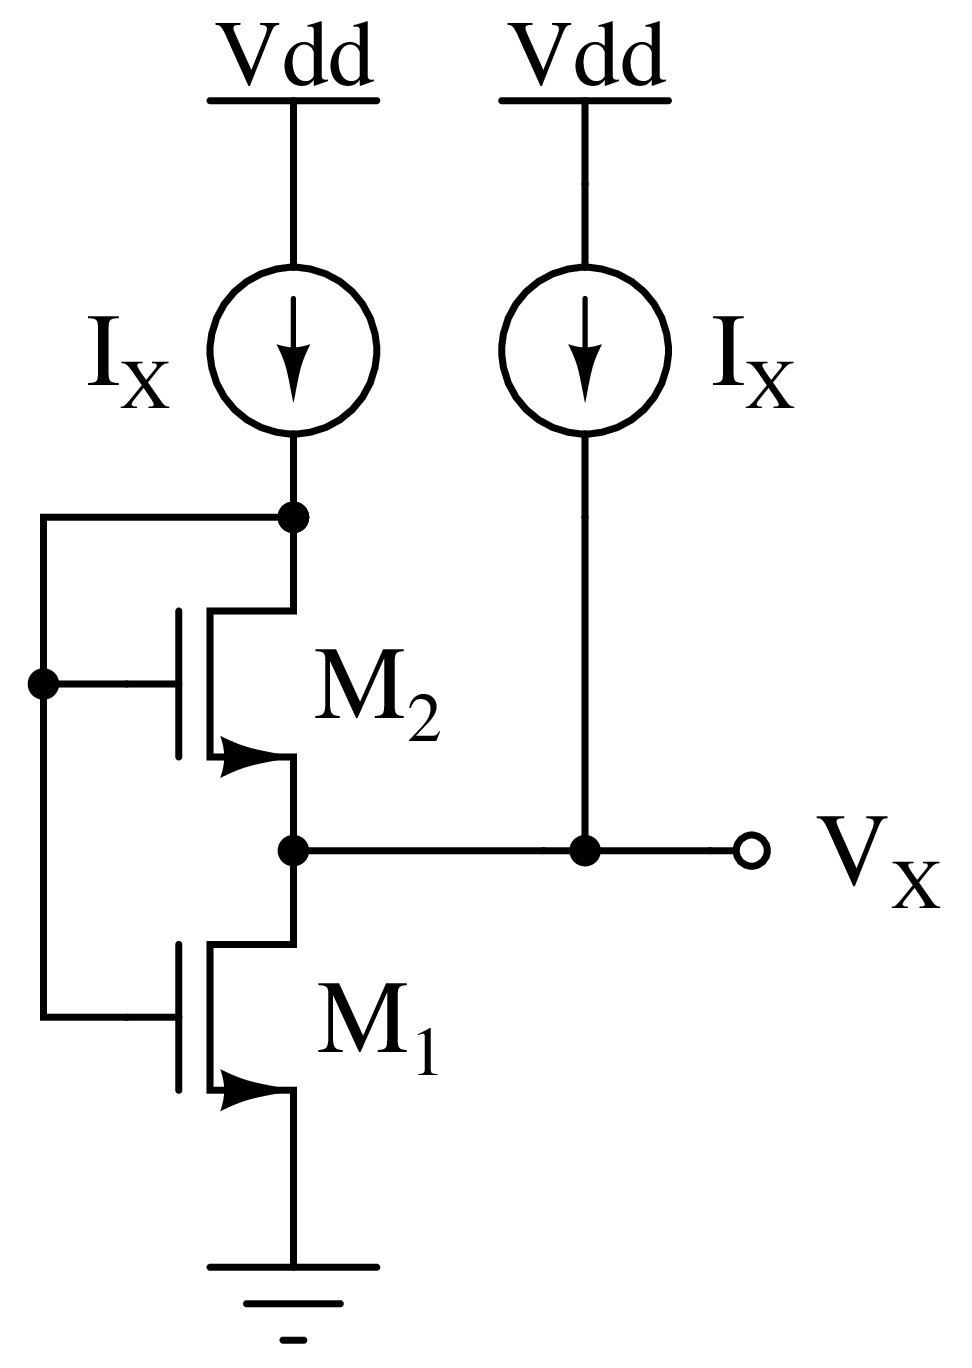
\includegraphics[width=0.25\textwidth]{Imagens/scm_circuit.jpg}
    \caption{Diagrama da estrutura \acrshort{scm}.}
    \label{fig:scm_circuit}
\end{wrapfigure}

Como $V_{DG1}=V_{SG2}$, vamos ter $i_{r1}=i_{f2}$. Além disso, como temos $V_{GD2}=0$, também teremos $i_{r2}=0$.

Equacionando as correntes que passam por cada um dos transistores:

\begin{equation}
    \label{eq:scm_m1_current}
    2I_X=I_{SH}\cdot S_1\cdot\left(i_{f1}-i_{r1}\right)
\end{equation}

\begin{equation}
    \label{eq:scm_m2_current}
    I_X=I_{SH}\cdot S_2\cdot i_{f2}
\end{equation}

\noindent onde $I_{SH}$ é a corrente específica dos transistores (assumida a mesma para ambos) e $S_1$ e $S_2$ são as razões de aspecto de cada transistor.

Dividindo \eqref{eq:scm_m1_current} por \eqref{eq:scm_m2_current} e substituindo $i_{r1}=i_{f2}$, vamos obter a seguinte equação:

\begin{equation}
    \label{eq:scm_m1_over_m2_current}
    2=\frac{S_1\cdot\left(i_{f1}-i_{f2}\right)}{S_2\cdot i_{f2}}
\end{equation}

Substituindo $i_{f1}=\alpha_{12}\cdot i_{f2}$ em \eqref{eq:scm_m1_over_m2_current} e isolando $\alpha_{12}$ nós obtemos

\begin{equation}
    \label{eq:scm_alpha}
    \alpha_{12}=1+2\cdot\frac{S_2}{S_1}
\end{equation}

Podemos ver de \eqref{eq:scm_alpha} que a razão entre $i_{f1}$ e $i_{f2}$ é uma constante,\endnote{A razão entre $i_{f1}$ e $i_{f2}$ depende das razões de aspecto dos transistores $S_1$ e $S_2$, mas esses parâmetros não variam durante a operação do circuito. Uma vez decididas as razões de aspecto durante o projeto, $\alpha_{12}$ é fixado e inalterável.} isto é, ao especificarmos $i_{f2}$, $i_{f1}$ é implicitamente fixo também. Por isso, vamos nos referir ao nível de inversão do transistor superior ($i_{f2}$) como nível de inversão do \acrshort{scm} como um todo.

Vamos utilizar \eqref{eq:scm_alpha} na próxima seção quando estivermos projetando o núcleo da fonte de corrente mas, antes disso, vamos aplicar as equações do \acrfull{uicm}\endnote{O desenvolvimento das equações do \acrshort{uicm} pode ser encontrado em \cite{acm:book}.} no \acrshort{scm}. Para isso, precisamos definir a seguinte função:

\begin{equation}
    \label{eq:uicm_function}
    F(i)=\sqrt{1+i}+\ln\left(\sqrt{1+i}-1\right)-2
\end{equation}


Aplicando as equações do \acrshort{uicm} nos transistores $M_1$ e $M_2$ podemos chegar na seguinte expressão:

\begin{equation}
    \label{eq:scm_uicm}
    V_X=\phi_t\left[F(\alpha_{12}\cdot i_{f2})-F(i_{f2})\right]
\end{equation}

\noindent que, se lembramos de \eqref{eq:scm_m2_current}, nos permite escrever $V_X$ em função de $I_X$ da seguinte forma:

\begin{equation}
    \label{eq:vx_de_ix}
    V_X(I_X)=\phi_t\left[F\left(\frac{\alpha_{12}\cdot I_X}{I_{SH}\cdot S_2}\right)-F\left(\frac{I_X}{I_{SH}\cdot S_2}\right)\right]
\end{equation}

Para fim de ilustração, a figura \ref{fig:scm_single_plot} mostra o gráfico de \eqref{eq:vx_de_ix} para os valores $I_{SH}=\sis{150}{\nano\ampere}$, $\alpha_{12}=2$ e $S_2=\num{0.01}$.

\begin{figure}[htp!]
    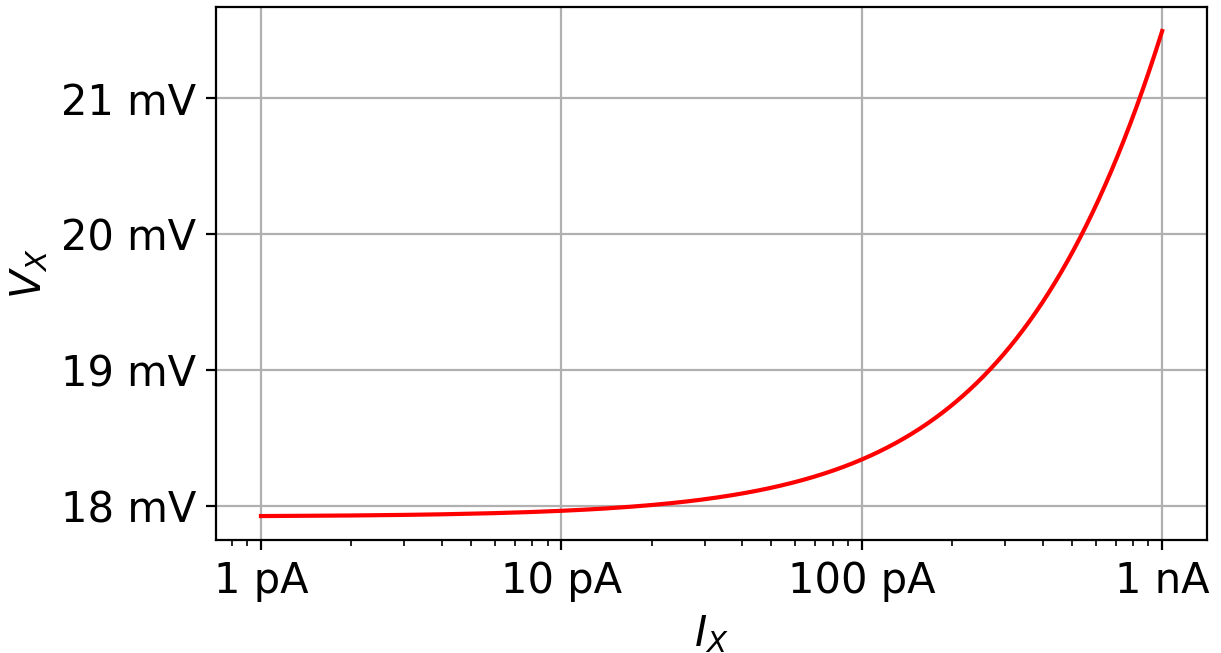
\includegraphics[width=\mysize\linewidth]{Imagens/scm_single_plot.png}
    \centering
    \caption{Gráfico da equação \eqref{eq:vx_de_ix}.}
    \label{fig:scm_single_plot}
\end{figure}

Vamos utilizar \eqref{eq:scm_alpha} e \eqref{eq:scm_uicm} para o projeto do núcleo da fonte de corrente e vamos utilizar \eqref{eq:vx_de_ix} para plotar as curvas associadas ao projeto.

\section{Projeto do núcleo da fonte de corrente}

Até então nós consideramos a estrutura \acrshort{scm} como uma fonte de tesão controlada por corrente, isto é, $V_X=f(I_X)$, mas nada nos impede de considerar a relação de forma inversa, isto é, $I_X=g(V_X)$.\endnote{Estamos assumindo que a função $f(\cdot)$ é uma função injetiva de forma que exista $g(\cdot)=f^{-1}(\cdot)$. Quais são as funções não é de importância, o importante é que existe um mapeamento um para um entre $I_X$ e $V_X$.} Vamos gerar essa tensão $V_X$ através de outro SCM (com transistores $M_3$ e $M_4$ no lugar de $M_1$ e $M_2$ respectivamente) que tenha a mesma corrente $I_X$. Vamos nos referir ao primeiro \acrshort{scm} por $\text{\acrshort{scm}}_{12}$ e ao segundo por $\text{\acrshort{scm}}_{34}$.

Se $\text{\acrshort{scm}}_{34}$ for idêntico a $\text{\acrshort{scm}}_{12}$, a restrição de mesma corrente $I_X$ e mesma tensão $V_X$ será respeitada para qualquer par $(I_X,V_X)$. Por esse motivo, vamos escolher razões de aspecto diferentes, para que a intersecção das curvas dos dois \acrshort{scm}s seja um único ponto e ele seja o ponto de operação desejado.

Os transistores $M_1$, $M_2$, $M_3$ e $M_4$ vão ser constituídos de associações em série ou paralelo de transistores unitários. O transistor unitário (vamos nos referenciar a ele por $M_0$) vai ter dimensões $W=\sis{220}{\nano\meter}$ e $L=\sis{19.995}{\micro\meter}$, que são as dimensões extremas ($W$ mínimo e $L$ máximo) da tecnologia $\sis{180}{\nano\meter}$ da \acrshort{tsmc}.\endnote{As dimensões extremas foram escolhidas depois de certa tentativa e erro para que as associações de transistores não envolvam quantidades absurdas de transistores.} A tensão de limiar foi extraída seguindo a metodologia apresentada em \cite{vt:extract} e a partir das equações apresentadas em \cite{acm:book} a corrente específica de folha $I_{SH}$ foi calculada.

\subsection{Equações de projeto}

Nesta subseção vamos desenvolver as equações de projeto do núcleo da fonte de corrente. Os resultados numéricos intermediários serão apesentados para fins ilustrativos mas todas as equações foram implementadas em um programa \texttt{Python} que extrai $I_{SH}$ através de dados de simulação e calcula diretamente (sem os arredondamentos intermediários necessários para colocar os valores neste relatório) as razões de aspecto dos transistores, além de como associar o transistor unitário para alcançar tais razões de aspecto.

Como temos mais graus de liberdades do que restrições de projeto, vamos definir algumas variáveis. Primeiro, vamos definir os níveis de inversão de cada \acrshort{scm} no ponto de operação. Vamos colocar $\text{\acrshort{scm}}_{12}$ em inversão moderada com $i_{f2}=10$ e $\text{\acrshort{scm}}_{34}$ em inversão fraca com $i_{f4}=\num{0.01}$. Vamos também fixar $\alpha_{12}=2$. A corrente alvo vai ser $I_X=\sis{20}{\pico\ampere}$ que vai ser posteriormente reduzida por um espelho de corrente e a corrente de folha extraída foi $I_{SH}=\sis{139.97}{\nano\ampere}$. Quando não especificado, a temperatura é assumida $\sis{26.85}{\celsius}$.

Aplicando \eqref{eq:scm_m2_current} em $\text{\acrshort{scm}}_{12}$ podemos chegar em

\begin{equation}
    \label{eq:sbcs_s2}
    S_2=\frac{I_X}{I_{SH}\cdot i_{f2}}\approx\num{1.429e-5}
\end{equation}

Através de \eqref{eq:scm_alpha} aplicada em $\text{\acrshort{scm}}_{12}$ podemos isolar e calcular $S_1$:

\begin{equation}
    \label{eq:sbcs_s1}
    S_1=\frac{2S_2}{\alpha_{12}-1}\approx\num{2.858e-5}
\end{equation}

Utilizando \eqref{eq:scm_uicm} aplicada em $\text{\acrshort{scm}}_{12}$ podemos calcular $V_X$:

\begin{equation}
    \label{eq:sbcs_vx}
    V_X=\phi_t\left[F(\alpha_{12}\cdot i_{f2})-F(i_{f2})\right]\approx\sis{43.99}{\milli\volt}
\end{equation}

Aplicando \eqref{eq:scm_uicm} em $\text{\acrshort{scm}}_{34}$ e lembrando que $V_X$ é o mesmo para ambos os \acrshort{scm}s, podemos calcular $\alpha_{34}$ numericamente:

\begin{equation}
    \label{eq:sbcs_a24}
    V_X=\phi_t\left[F(\alpha_{34}\cdot i_{f4})-F(i_{f4})\right]
    \quad\Rightarrow\quad
    \alpha_{34}\approx\num{5.425}
\end{equation}

Por analogia, podemos repetir \eqref{eq:sbcs_s2} e \eqref{eq:sbcs_s1} em $\text{\acrshort{scm}}_{34}$ para obtermos $S_3$ e $S_4$:

\begin{equation}
    \label{eq:sbcs_s4}
    S_4=\frac{I_X}{I_{SH}\cdot i_{f4}}\approx\num{1.429e-2}
\end{equation}

\begin{equation}
    \label{eq:sbcs_s3}
    S_3=\frac{2S_4}{\alpha_{34}-1}\approx\num{6.459e-3}
\end{equation}

Temos todas as razões de aspecto dos transistores dos dois \acrshort{scm}s. A figura \ref{fig:scm_teorico} mostra o gráfico de \eqref{eq:vx_de_ix} para ambos os \acrshort{scm}s onde podemos identificar o ponto de operação em $I_X\approx\sis{20.08}{\pico\ampere}$ e $V_X\approx\sis{44.03}{\milli\volt}$, em concordância com as equações de projeto.

\begin{figure}[htp!]
    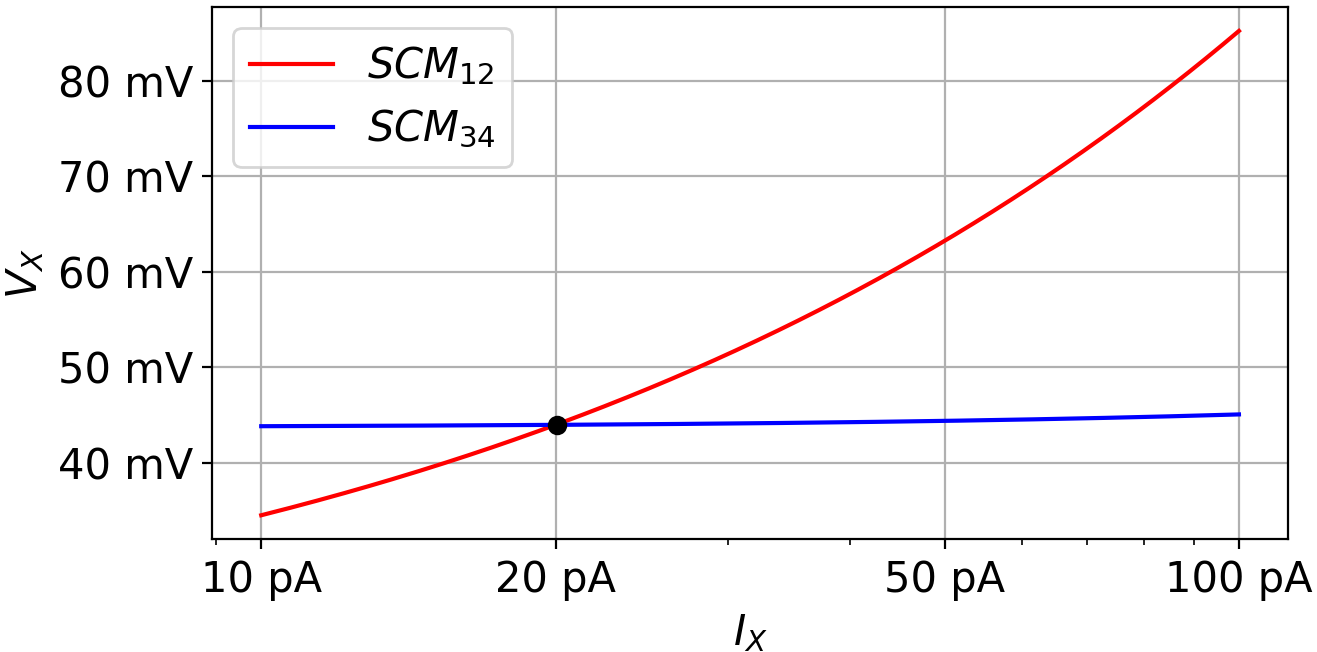
\includegraphics[width=\mysize\linewidth]{Imagens/scm_teorico.png}
    \centering
    \caption{Curvas características teóricas de $\text{\acrshort{scm}}_{12}$ e $\text{\acrshort{scm}}_{34}$.}
    \label{fig:scm_teorico}
\end{figure}

\subsection{Associações do transistor unitário}

Para alcançarmos as razões de aspecto calculadas, vamos associar $M_0$ com $W=\sis{220}{\nano\meter}$ e $L=\sis{19.995}{\micro\meter}$. $M_1$ vai ser a associação em série de 385 transistores $M_0$, nos resultando na seguinte razão de aspecto:

\begin{equation}
    \label{eq:associacao_s1}
    S_1'=\frac{W}{385\cdot L}\approx\num{2.858e-5}
\end{equation}

\noindent um valor que difere de \eqref{eq:sbcs_s1} em $\sis{0.0035}{\percent}$.

$M_2$ vai ser uma associação de 770 transistores $M_0$ em série, resultando na seguinte razão de aspecto:

\begin{equation}
    \label{eq:associacao_s2}
    S_2'=\frac{W}{770\cdot L}\approx\num{1.429e-5}
\end{equation}

\noindent um valor que difere de \eqref{eq:sbcs_s2} em $\sis{0.0035}{\percent}$.

$M_3$ vai ser uma associação de 2 transistores $M_0$ em série, resultando na seguinte razão de aspecto:

\begin{equation}
    \label{eq:associacao_s3}
    S_3'=\frac{W}{2\cdot L}\approx\num{5.501e-3}
\end{equation}

\noindent um valor que difere de \eqref{eq:sbcs_s3} em $\sis{14.82}{\percent}$.

Por fim, $M_4$ vai ser simplesmente $M_0$, resultando na seguinte razão de aspecto:

\begin{equation}
    \label{eq:associacao_s4}
    S_4'=\frac{W}{L}\approx\num{1.101e-2}
\end{equation}

\noindent um valor que difere de \eqref{eq:sbcs_s4} em $\sis{23}{\percent}$.

Os erros associados a $S_3$ e $S_4$ se mostraram consideravelmente altos. Isso se dá pelo fato de usarmos associações apenas em série ou apenas em paralelo\endnote{A decisão de não misturar associações em série e em paralelo foi feita com objetivo de se manter o projeto relativamente simples. Como é descrito no texto logo em seguida, as discrepâncias acabam sendo vantajosas.} e, nesses dois casos na qual a quantidade de transistores utilizada é baixa, os erros tendem a aumentar. Mas, pelo fato de ambos os valores terem sido menores do que os esperados, podemos ver de \eqref{eq:vx_de_ix} que isso vai tender a diminuir $I_X$, o que nos facilita a vida posteriormente.

\subsection{Simulações dos \acrshort{scm}s com fontes de corrente ideais}

Vamos traçar as curvas características dos \acrshort{scm}s através da simulação, utilizando as fontes de corrente ideais. Tais curvas podem ser vistas na figura \ref{fig:scm_simulado} onde podemos verificar o ponto de operação em $I_X\approx\sis{14.14}{\pico\ampere}$ e $V_X\approx\sis{43.32}{\milli\volt}$.

\begin{figure}[htp!]
    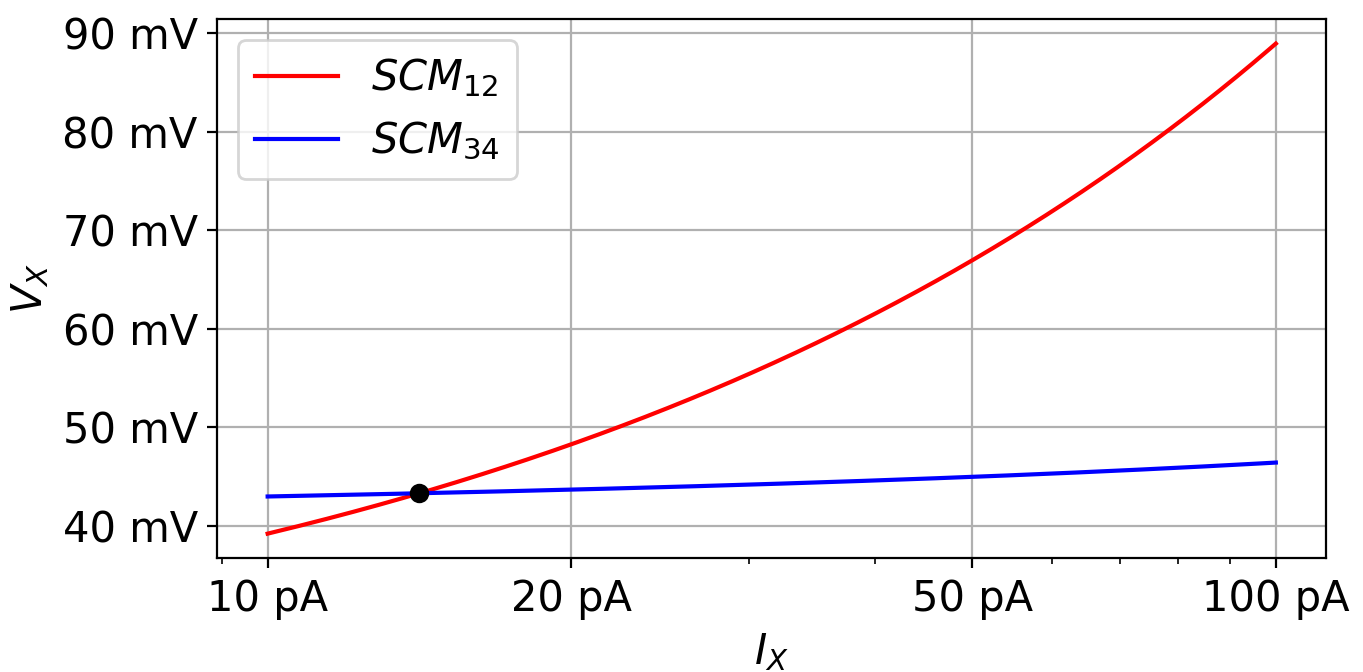
\includegraphics[width=\mysize\linewidth]{Imagens/scm_simulado.png}
    \centering
    \caption{Curvas características simuladas de $\text{\acrshort{scm}}_{12}$ e $\text{\acrshort{scm}}_{34}$.}
    \label{fig:scm_simulado}
\end{figure}

O valor de $V_X$ deu extremamente próximo do valor teórico, diferindo em apenas $\sis{0.26}{\percent}$. Como previsto, as discrepâncias entre as razões de aspecto de $\text{\acrshort{scm}}_{34}$ resultaram numa diminuição da corrente em $\sis{29.58}{\percent}$.

\pagebreak

\section{Simulações do núcleo}

\begin{wrapfigure}[8]{r}{0.35\textwidth}
    \centering
    \vspace{-0.5cm}
    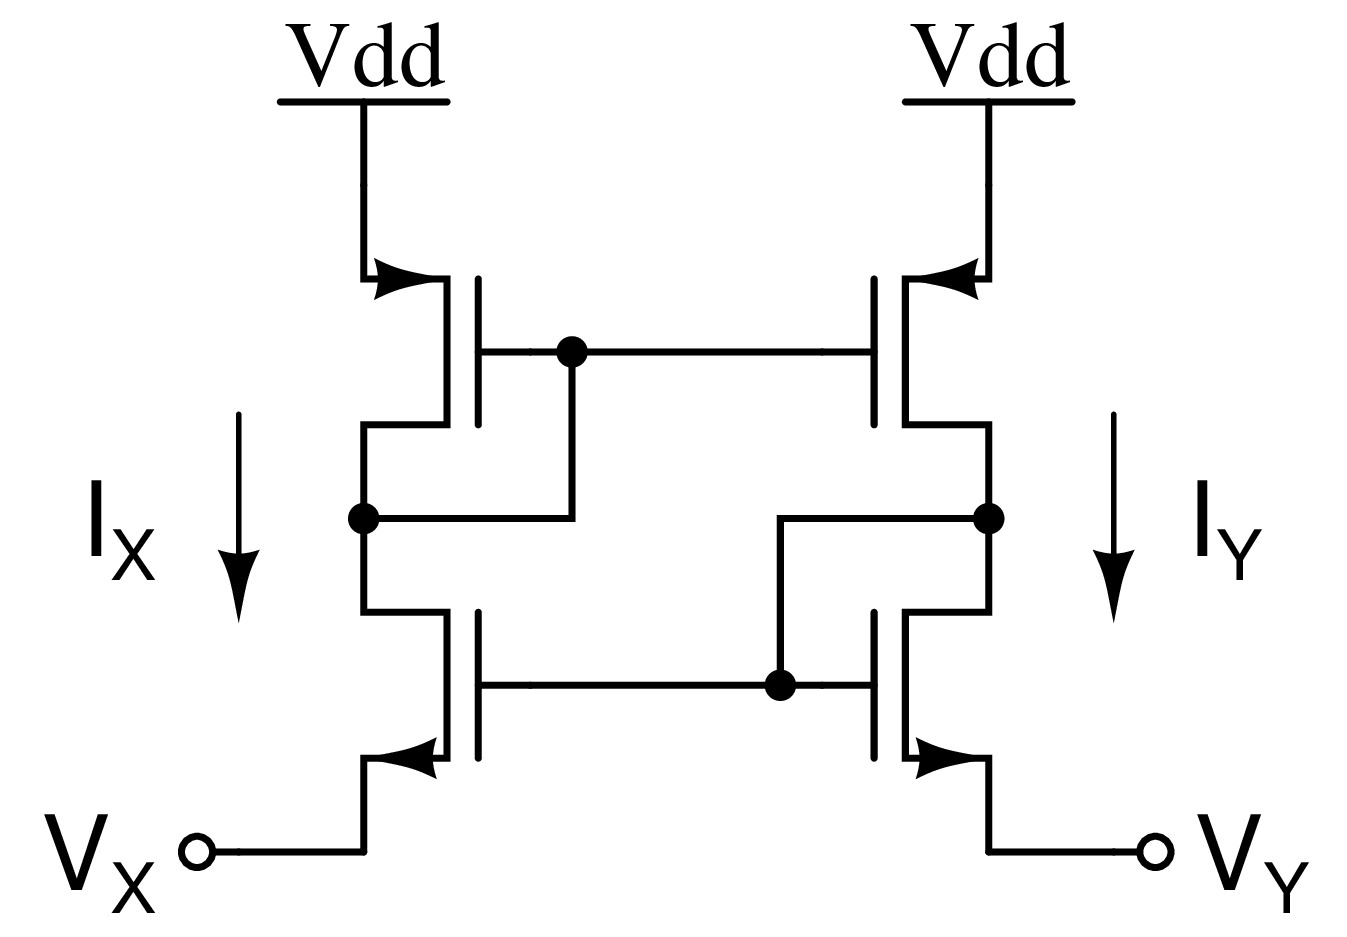
\includegraphics[width=0.35\textwidth]{Imagens/vfcm_simple_circuit.jpg}
    \caption{Circuito \acrshort{vfcm}.}
    \label{fig:vfcm_simple_circuit}
\end{wrapfigure}

Para podermos garantir que as tensões e correntes de ambos os \acrshort{scm}s sejam iguais, vamos precisar de uma estrutura chamada \acrfull{vfcm}. A topologia de um \acrshort{vfcm} simples é apresentada na figura \ref{fig:vfcm_simple_circuit}. Utilizando a dedução apresentada em \cite{sbcs} vemos que, quando os ramos esquerdo e direito apresentam transistores idênticos, temos $V_X=V_Y$ e $I_X=I_Y$, exatamente o que precisamos.

\begin{figure}[htp!]
    \centering
    \subfigure[Núcleo simples.]{
    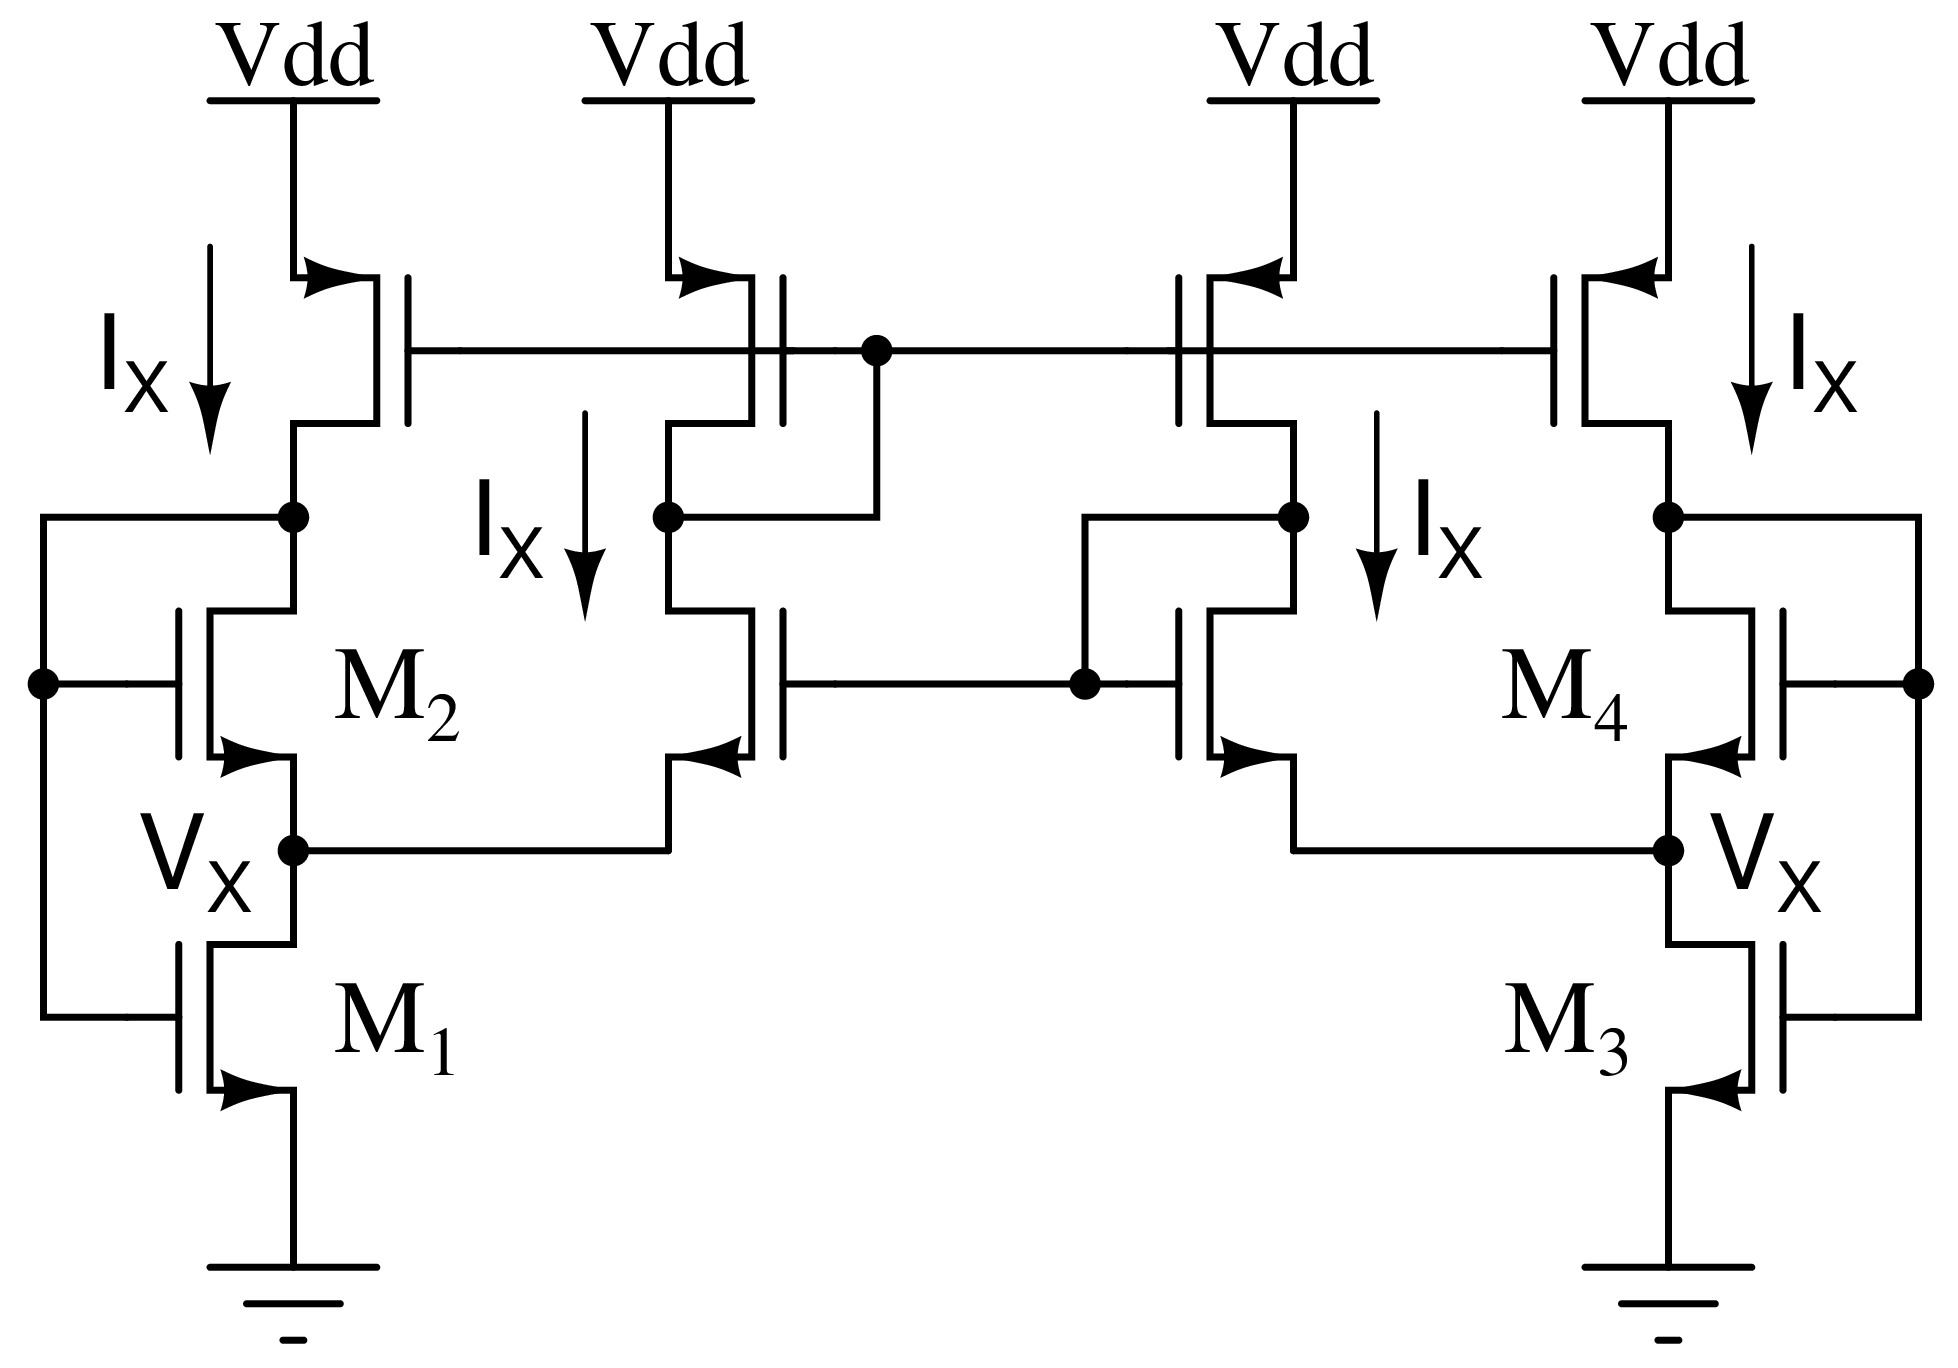
\includegraphics[width=0.39\textwidth]{Imagens/sbcs_simple_circuit.jpg}
    \label{fig:sbcs_simple_circuit}
    }
    \hspace{1.5cm}
    \subfigure[Núcleo modificado.]{
    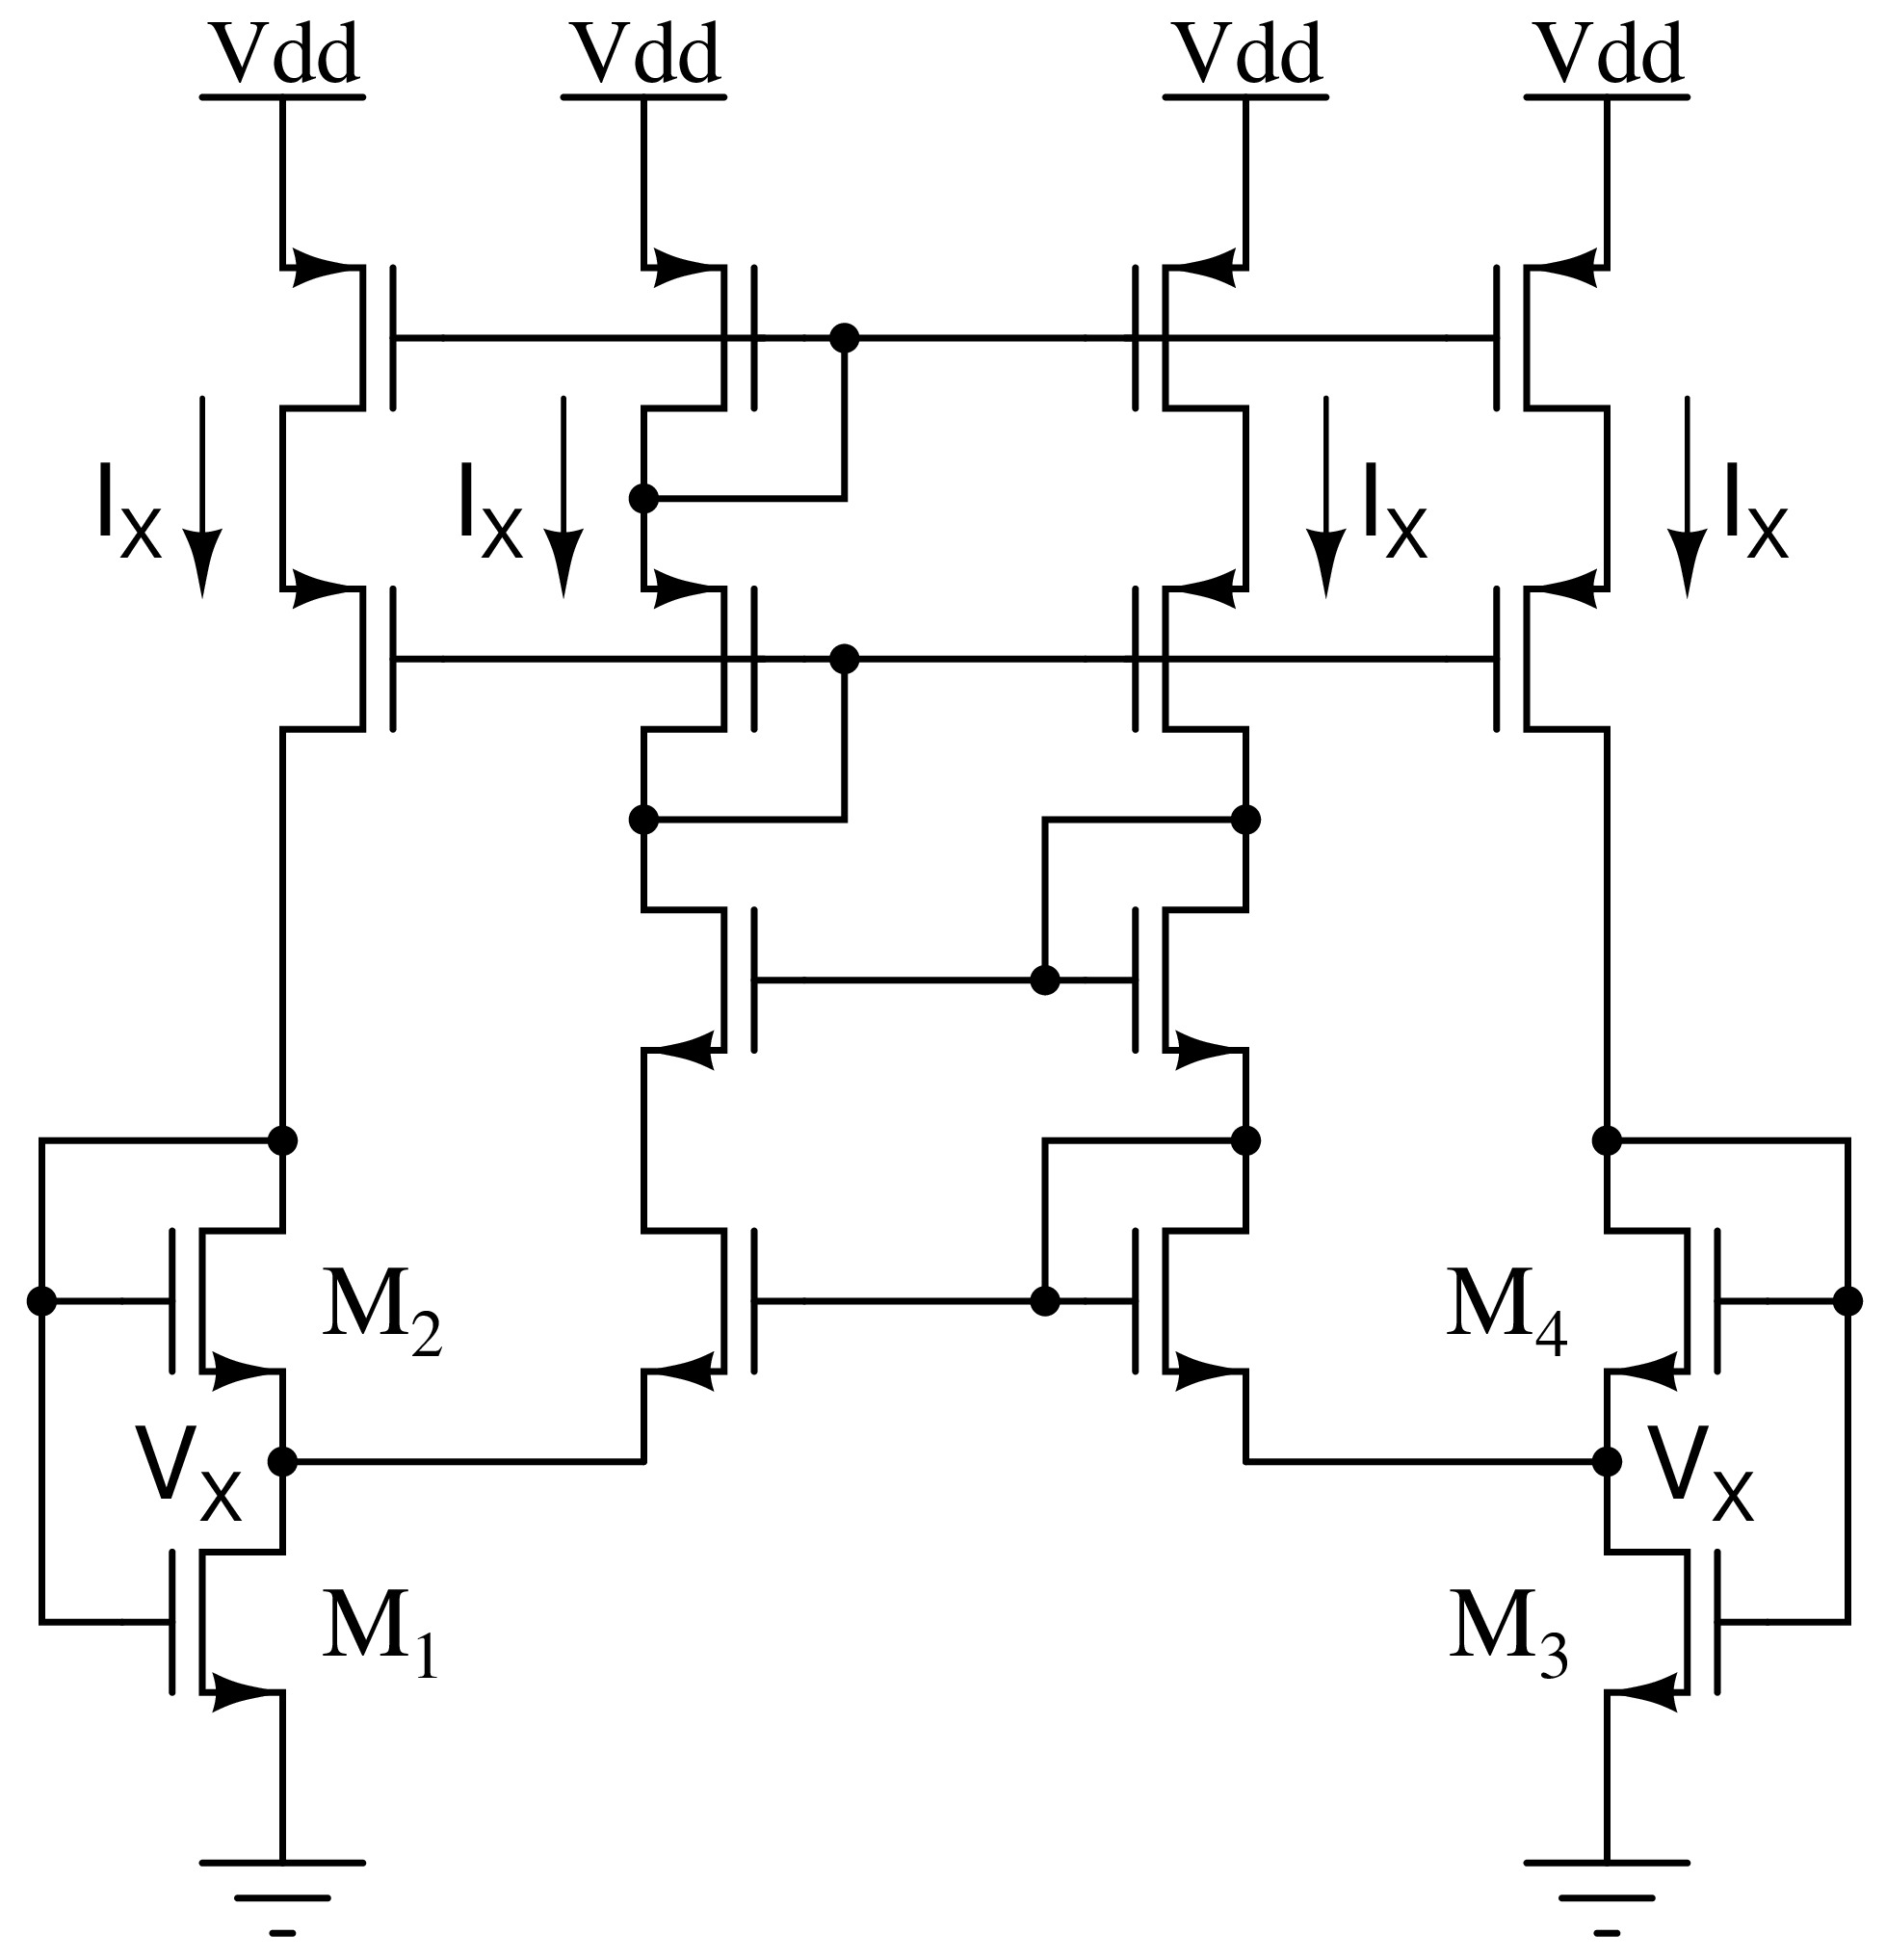
\includegraphics[width=0.39\textwidth]{Imagens/sbcs_cascoded_circuit.jpg}
    \label{fig:sbcs_cascoded_circuit}
    }
    \caption[Diferentes topologias para o núcleo da fonte de corrente.]{Diferentes topologias para o núcleo da fonte de corrente. Imagens \subref{fig:sbcs_simple_circuit} e \subref{fig:sbcs_cascoded_circuit} mostram respectivamente as estruturas simples e modificada do núcleo da fonte de corrente.}
    \label{fig:core_topology}
\end{figure}

Podemos ver na figura \ref{fig:sbcs_simple_circuit} o núcleo simples apresentado em \cite{sbcs} e na figura \ref{fig:sbcs_cascoded_circuit} uma versão modificada que troca todos os espelhos simples por espelhos \textit{cascode}. A topologia da figura \ref{fig:sbcs_cascoded_circuit} é a que foi adotada neste trabalho.

Vamos analisar a regulação de linha do núcleo. A figura \ref{fig:core_vdd_sweep} mostra a corrente de referência para diferentes valores da tensão de alimentação. Na alimentação nominal de $\sis{1.8}{\volt}$ a corrente foi $I_X=\sis{14.6}{\pico\ampere}$, condizente com o valor obtido na figura \ref{fig:scm_simulado} e a potência consumida foi $\sis{104.4}{\pico\watt}$. A sensibilidade média\endnote{Vamos definir o que exatamente está sendo referido por sensibilidade média. Suponhamos que queremos medir a sensibilidade média de uma função $f(x)$ em relação à sua variável independente $x\in[a,b]$. Para isso, precisamos analisar a sensibilidade local que é definida da seguinte forma:

\begin{equation}
    \label{eq:delta_f}
    \delta f(x)=\frac{1}{f(x)}\cdot\deriv{f(x)}{x}{}=\frac{f'(x)}{f(x)}
\end{equation}

Como queremos a sensibilidade média, precisamos calcular o valor médio de $\delta f(x)$ em $x\in[a,b]$, que é dado pela seguinte integral:

\begin{equation}
    \label{eq:delta_f_mean}
    \overline{\delta f}=\frac{1}{b-a}\int_{a}^{b}\delta f(x)\,dx=\frac{1}{b-a}\int_{a}^{b}\frac{f'(x)}{f(x)}\,dx
\end{equation}

Adotando a substituição $u=f(x)$ podemos resolver a integral e chegar em um resultado que, quando expresso em porcentagem, assume a seguinte forma:

\begin{equation}
    \label{eq:delta_f_mean_solved}
    \overline{\delta f}=\frac{\sis{100}{\percent}}{b-a}\cdot\ln\abs{\frac{f(b)}{f(a)}}
\end{equation}

Toda vez que alguma sensibilidade média for citada ao longo do resto do texto, essa é a forma com a qual tal sensibilidade é calculada.} na faixa de $\sis{700}{\milli\volt}$ até $\sis{1.8}{\volt}$ foi de $\sis{3.24}{\percent\per\volt}$.

\begin{figure}[htp!]
    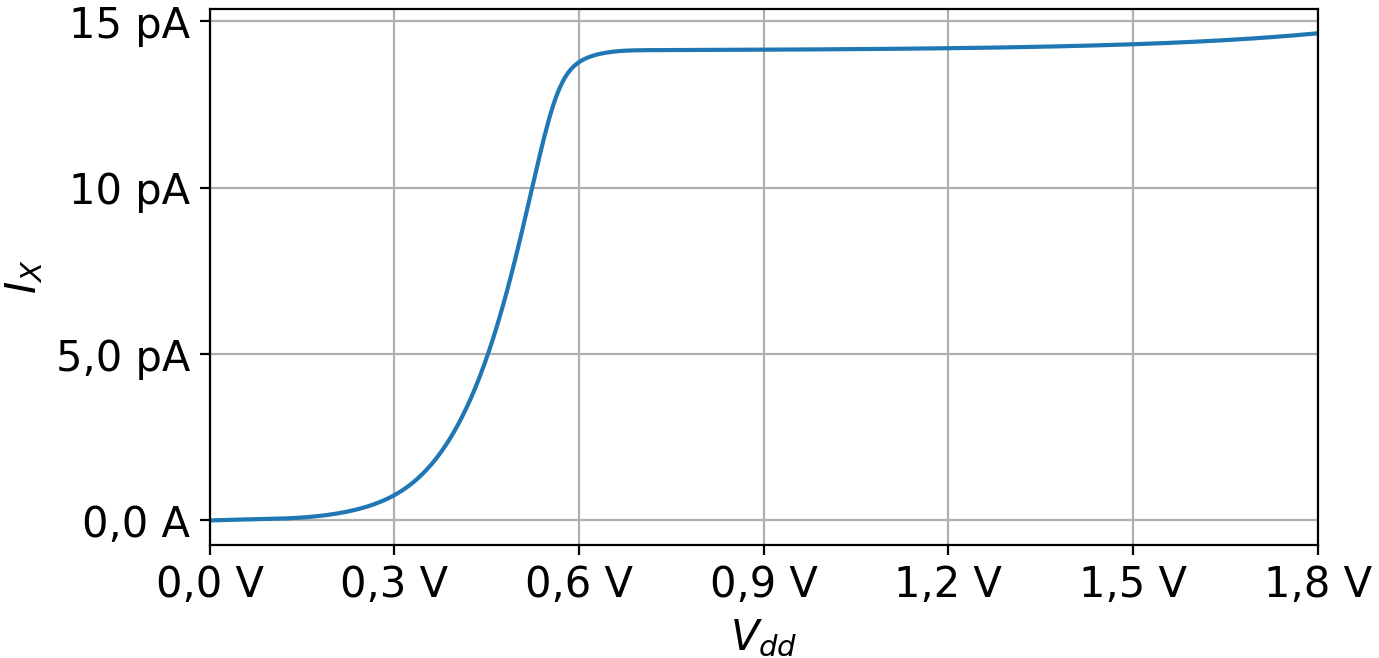
\includegraphics[width=\mysize\linewidth]{Imagens/core_vdd_sweep.png}
    \centering
    \caption{Gráfico da regulação de linha do núcleo.}
    \label{fig:core_vdd_sweep}
\end{figure} 

Vamos analisar a sensibilidade térmica do núcleo com a alimentação fixa em $\sis{1.8}{\volt}$. A figura \ref{fig:core_temp_sweep} mostra como a corrente $I_X$ varia com a temperatura. A sensibilidade média na faixa de $\sis{0}{\celsius}$ até $\sis{100}{\celsius}$ foi de $\sis{1.36}{\percent\per\celsius}$ e na faixa de $\sis{0}{\celsius}$ até $\sis{60}{\celsius}$ foi de $\sis{0.45}{\percent\per\celsius}$.

\begin{figure}[htp!]
    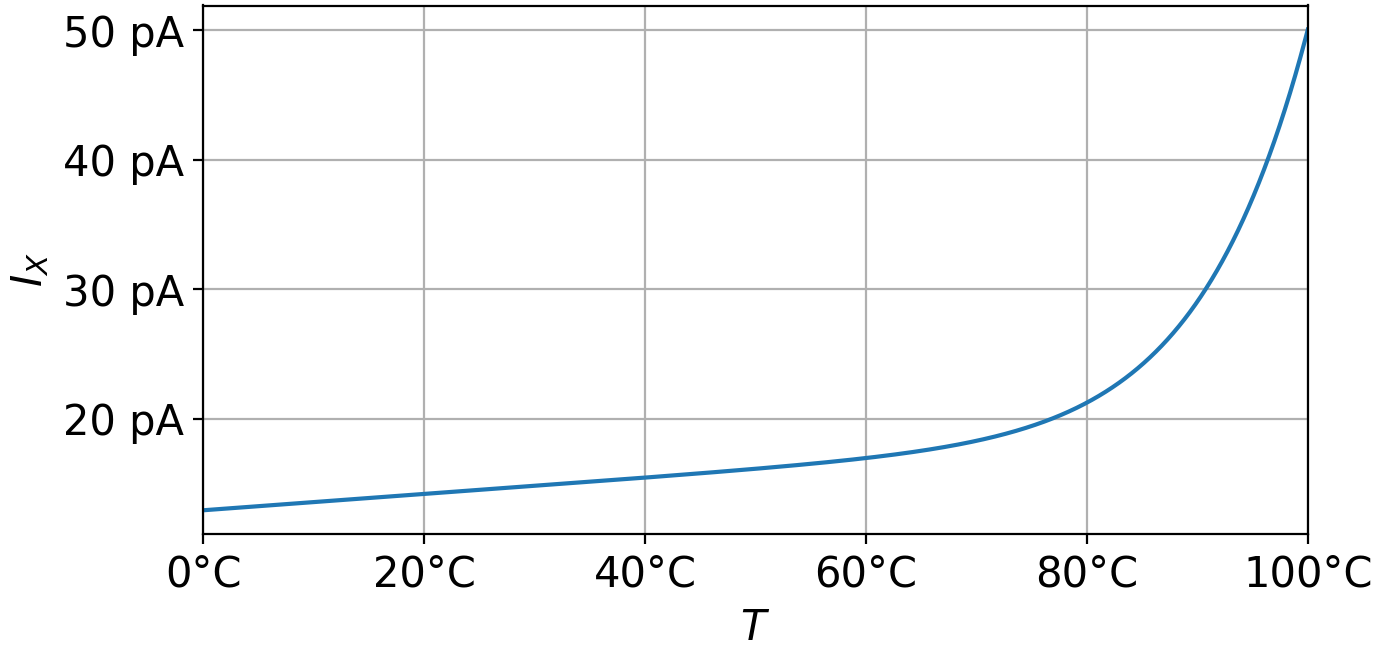
\includegraphics[width=\mysize\linewidth]{Imagens/core_temp_sweep.png}
    \centering
    \caption{Gráfico da sensibilidade térmica do núcleo para tensão de alimentação fixa em $V_{dd}=\sis{1.8}{\volt}$.}
    \label{fig:core_temp_sweep}
\end{figure}

\section{Fonte de corrente completa}

Nesta seção vamos apresentar a topologia completa da fonte de corrente além de demonstrar simulações de caracterização do circuito.

\subsection{Redução da corrente do núcleo}

\begin{wrapfigure}[11]{r}{0.4\textwidth}
    \centering
    \vspace{-0.5cm}
    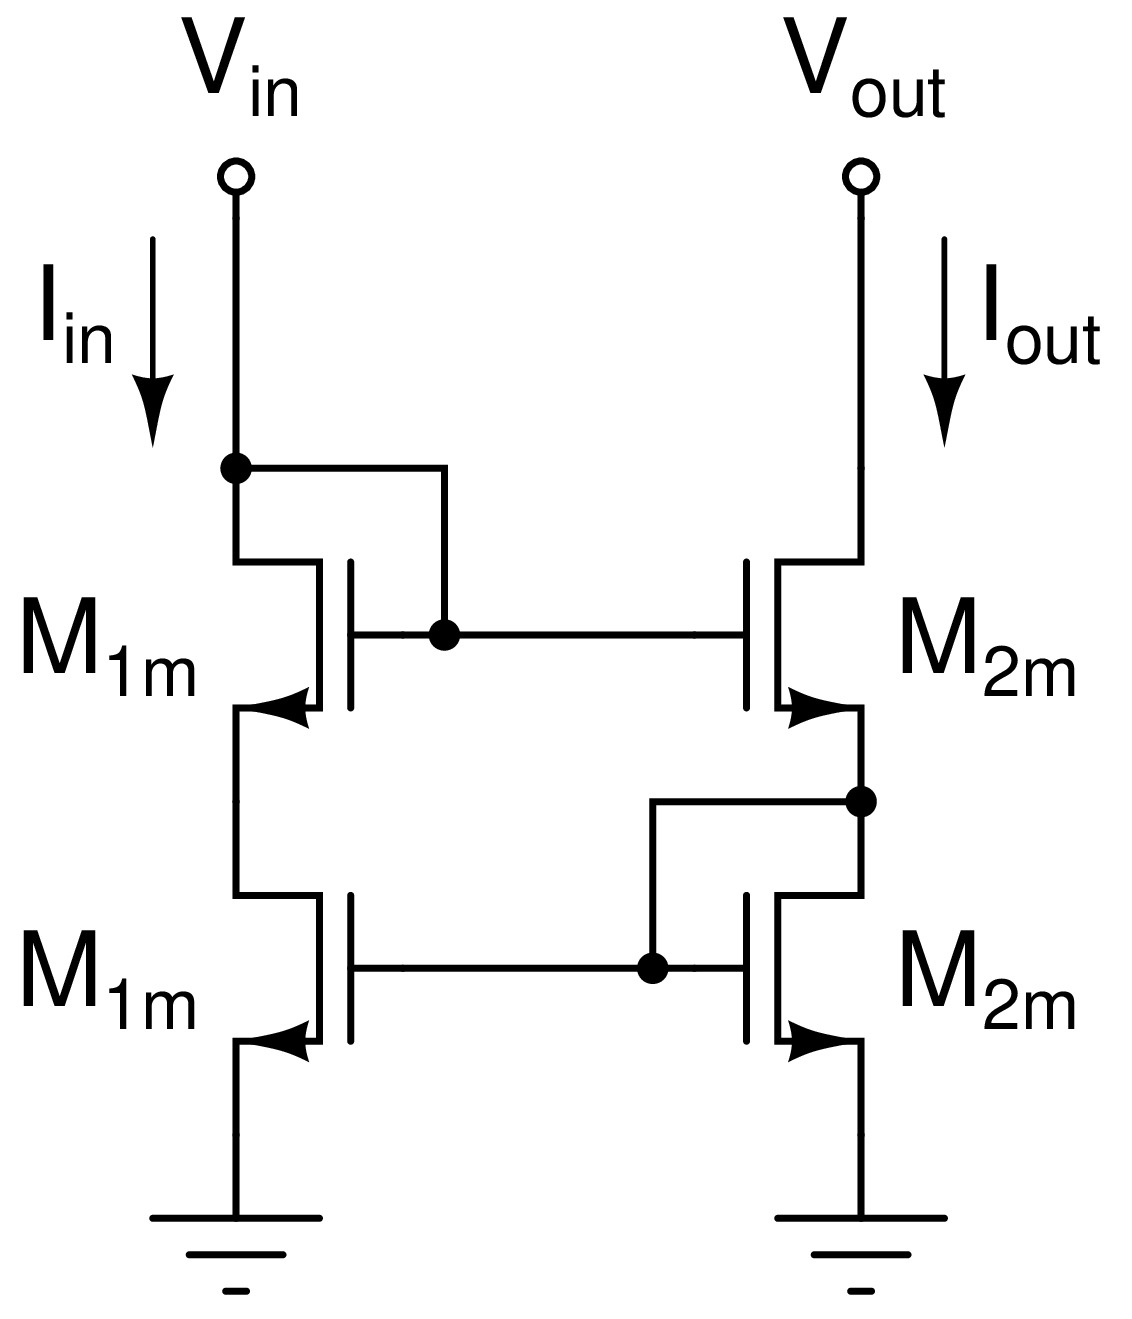
\includegraphics[width=0.28\textwidth]{Imagens/mirror.jpg}
    \caption{Espelho de corrente de Wilson melhorado com razão 15:1.}
    \label{fig:mirror}
\end{wrapfigure}

Temos uma referência de corrente de aproximadamente $\sis{15}{\pico\ampere}$. Para atingirmos o objetivo proposto de $\sis{1}{\pico\ampere}$, vamos cascatear o núcleo com um espelho de corrente de razão 15:1. A topologia utilizada é a apresentada em \cite{wilson} e reproduzida na figura \ref{fig:mirror}. Os transistores $M_{1m}$ são a associação de 5 transistores com $W=\sis{1}{\micro\meter}$ e $L=\sis{19.995}{\micro\meter}$ em paralelo e os transistores $M_{2m}$ são associações de 3 transistores de mesmas dimensões em série.

Cascateando o núcleo da figura \ref{fig:sbcs_cascoded_circuit} com o espelho de corrente da figura \ref{fig:mirror} resulta na fonte de corrente completa que pode ser vista na figura \ref{fig:full_sbcs}.

\begin{figure}[htp!]
    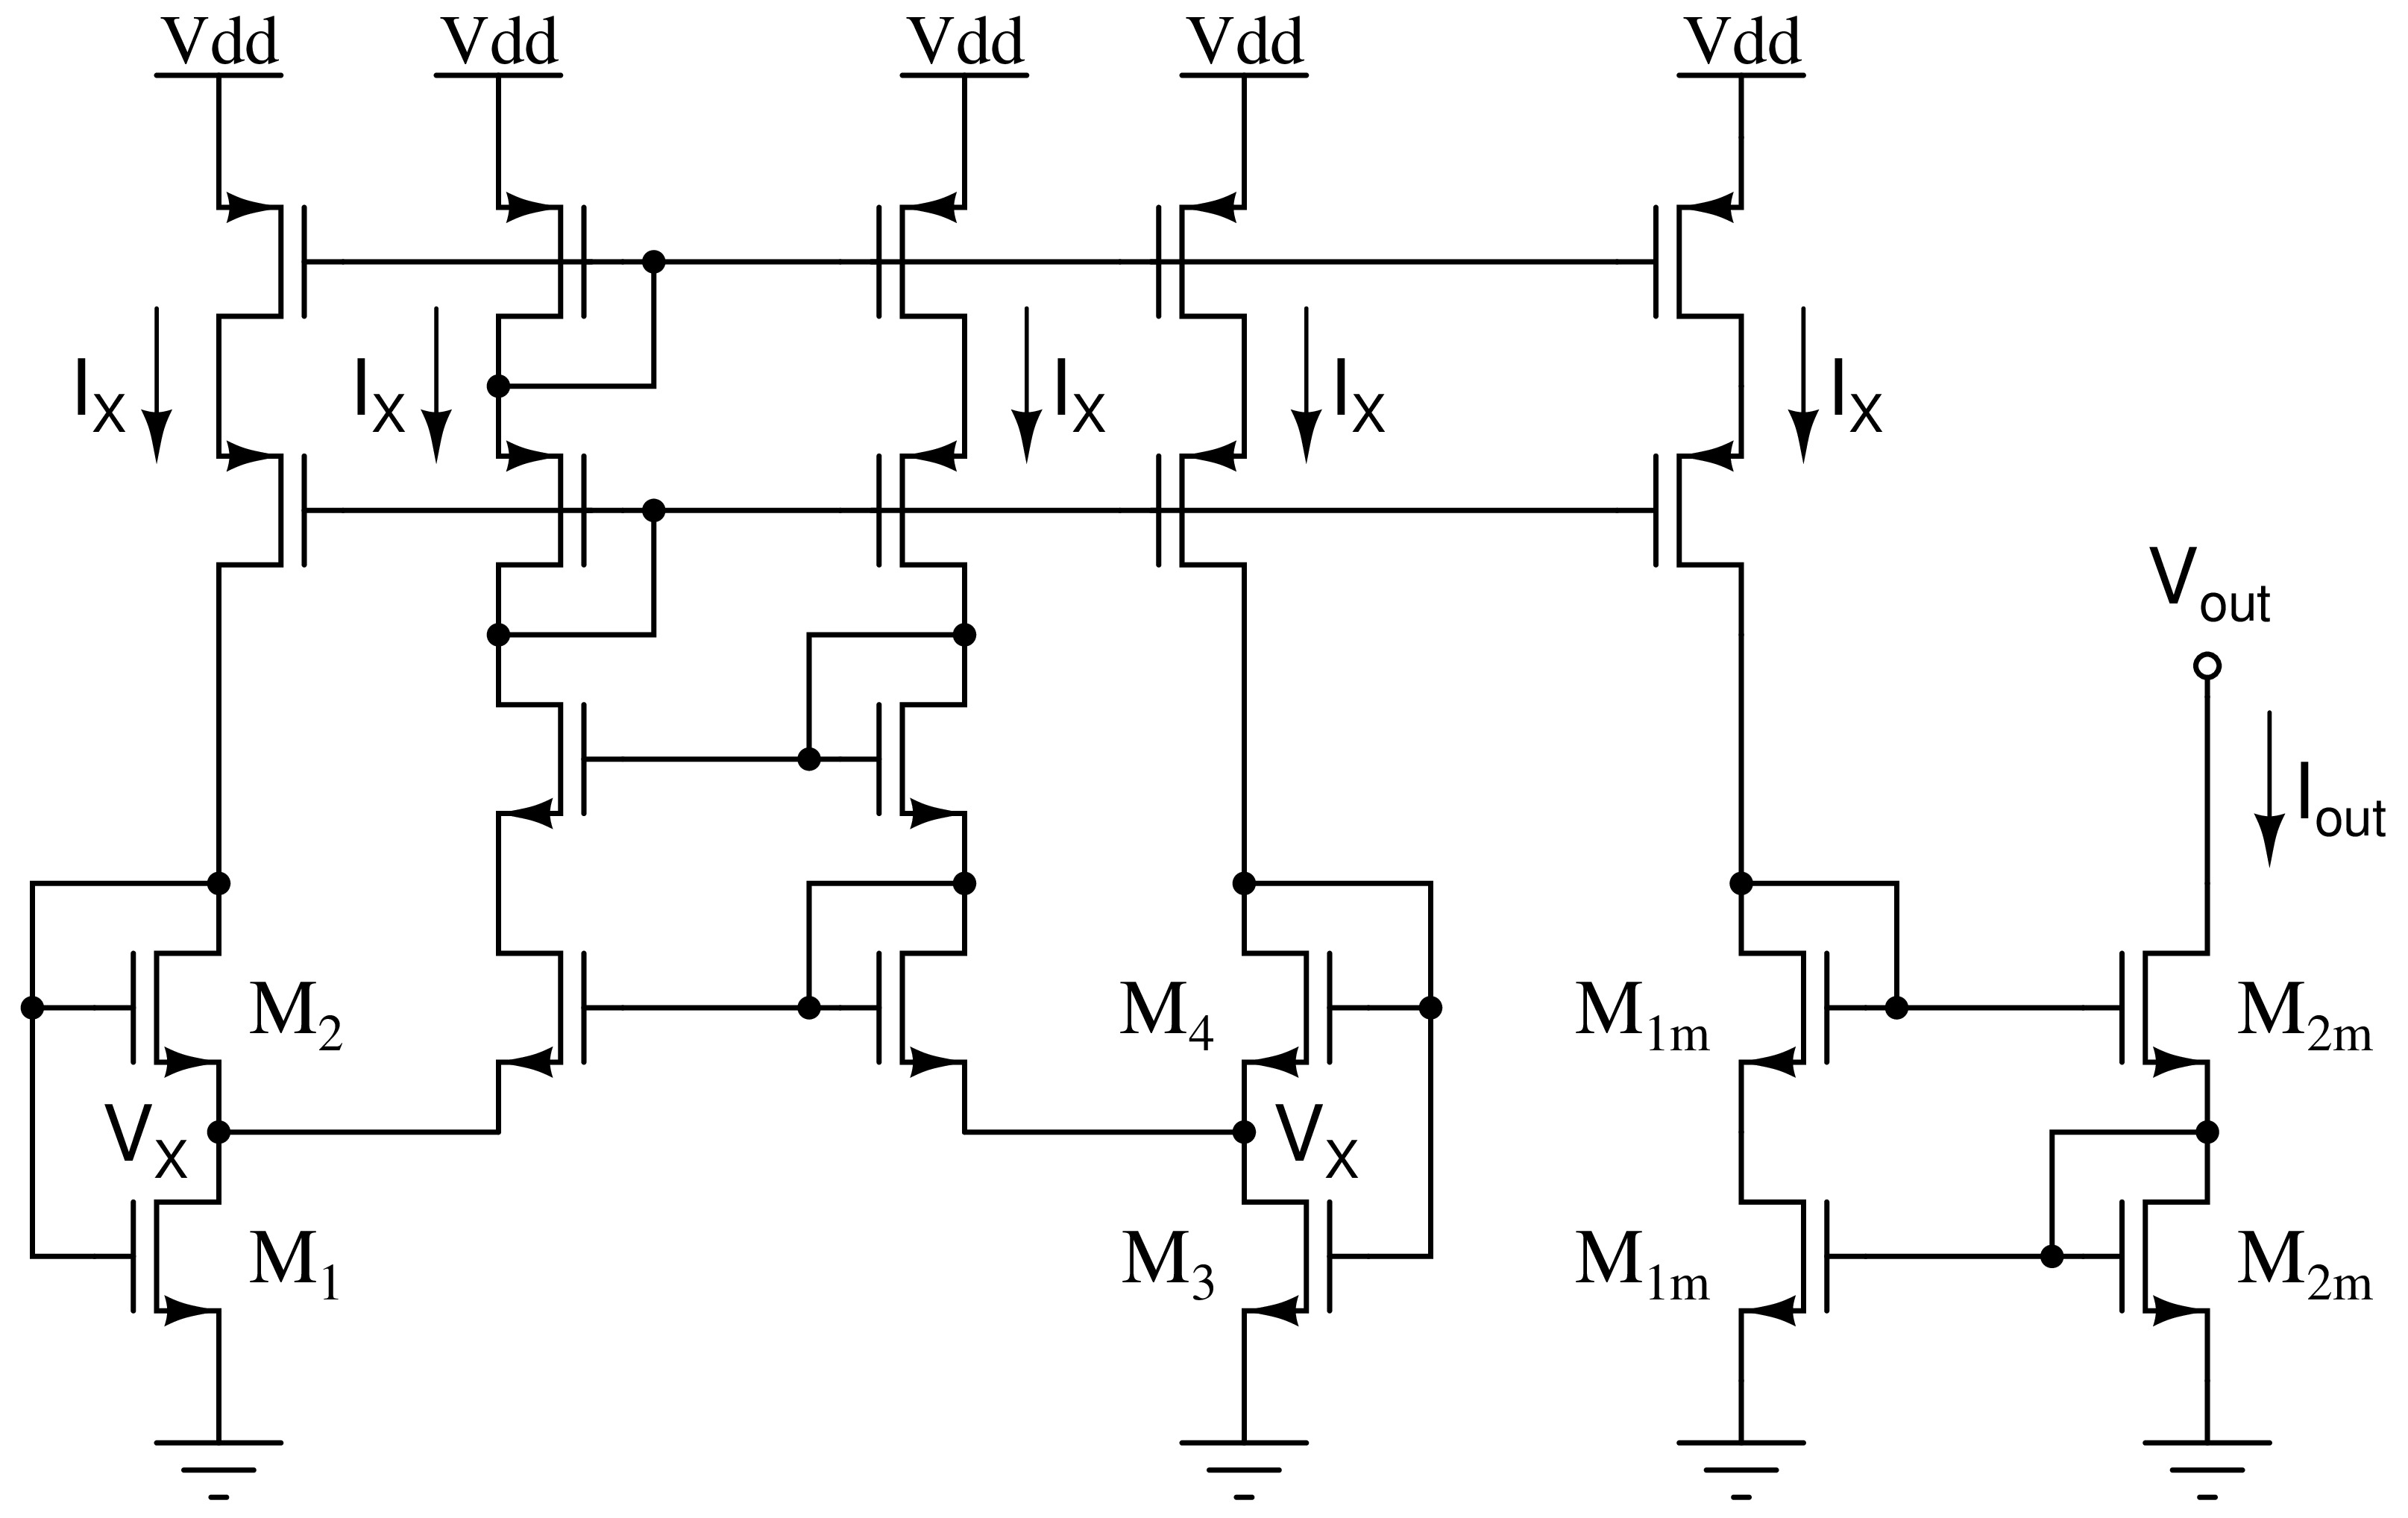
\includegraphics[width=\mysize\linewidth]{Imagens/full_sbcs.jpg}
    \centering
    \caption{Circuito completo da fonte de corrente.}
    \label{fig:full_sbcs}
\end{figure}

Vamos analisar as sensibilidades da fonte de corrente a variações na tensão de alimentação e temperatura.

\subsection{Simulações da fonte de corrente completa}

Vamos analisar a regulação de linha desta fonte de corrente variando a alimentação $V_{dd}$ de $\sis{0}{\volt}$ até $\sis{1.8}{\volt}$ para 6 valores diferentes de $V_{out}$. As cuvas da regulação de linha podem ser vistas na figura \ref{fig:mirror_vdd_sweep_vout_par}. Na tabela \ref{tab:iout_vdd_vout_par} podemos verificar a corrente de saída para alimentação nominal de $\sis{1.8}{\volt}$ e a sensibilidade média à alimentação na faixa de $\sis{700}{\milli\volt}$ até $\sis{1.8}{\volt}$ para cada uma das tensões de saída.

\begin{figure}[t!]
    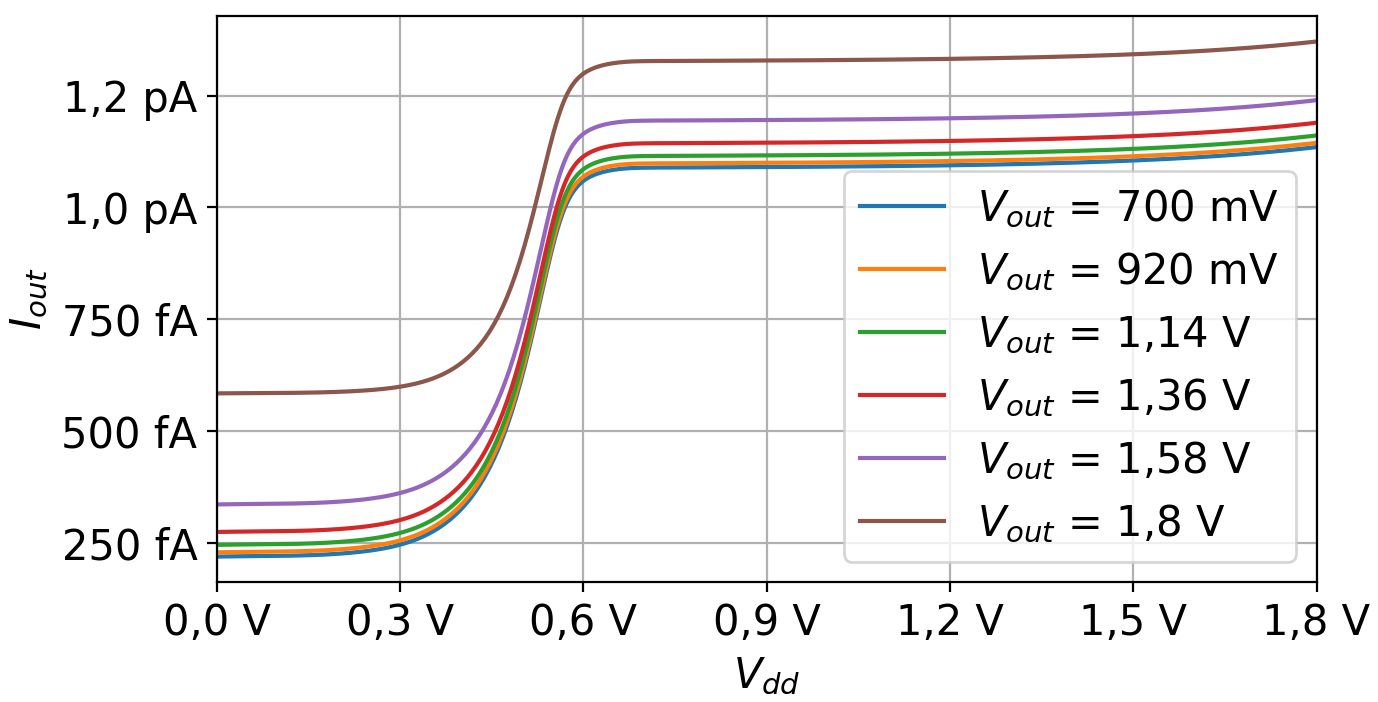
\includegraphics[width=\mysize\linewidth]{Imagens/mirror_vdd_sweep_vout_par.png}
    \centering
    \caption{Gráfico da regulação de linha da fonte completa para diferentes tensões de saída.}
    \label{fig:mirror_vdd_sweep_vout_par}
\end{figure}

\begingroup
\renewcommand{\arraystretch}{1.5}
\begin{table}[htp!]
    \centering
    \resizebox{\textwidth}{!}{
    \begin{tabular}{|
    >{\columncolor[HTML]{C0C0C0}}c |
    >{\columncolor[HTML]{FFFFFF}}c |
    >{\columncolor[HTML]{FFFFFF}}c |
    >{\columncolor[HTML]{FFFFFF}}c |
    >{\columncolor[HTML]{FFFFFF}}c |
    >{\columncolor[HTML]{FFFFFF}}c |
    >{\columncolor[HTML]{FFFFFF}}c |}
        \hline
        $V_{out}$ & \cellcolor[HTML]{FFFFFF}$\sis{700}{\milli\volt}$ & $\sis{920}{\milli\volt}$ & $\sis{1.14}{\volt}$ & $\sis{1.36}{\volt}$ & $\sis{1.58}{\volt}$ & $\sis{1.8}{\volt}$
        \\ \hline
        \cellcolor[HTML]{C0C0C0}$\eval{I_{out}}{V_{dd}=\sis{1.8}{\volt}}$ & $\sis{1.135}{\pico\ampere}$ & $\sis{1.144}{\pico\ampere}$ & $\sis{1.161}{\pico\ampere}$ & $\sis{1.189}{\pico\ampere}$ & $\sis{1.239}{\pico\ampere}$ & $\sis{1.371}{\pico\ampere}$
        \\ \hline
        $\overline{\delta I_{out}}$ & $\sis{3.77}{\percent\per\volt}$ & $\sis{3.74}{\percent\per\volt}$ & $\sis{3.68}{\percent\per\volt}$ & $\sis{3.59}{\percent\per\volt}$ & $\sis{3.43}{\percent\per\volt}$ & $\sis{2.96}{\percent\per\volt}$
        \\ \hline
    \end{tabular}
    }
    \caption{Tabela com as correntes de saída para alimentação nominal e sensibilidades médias em relação à alimentação de $\sis{700}{\milli\volt}$ até $\sis{1.8}{\volt}$ para diferentes valores da tensão de saída.}
    \label{tab:iout_vdd_vout_par}
\end{table}
\endgroup

Vamos analisar a sensibilidade térmica da fonte completa para a condição $V_{dd}=V_{out}=\sis{1.8}{\volt}$. A temperatura foi variada de $\sis{0}{\celsius}$ até $\sis{100}{\celsius}$. A figura \ref{fig:mirror_temp_sweep} nos mostra como a corrente de saída varia com a temperatura nas condições descritas. Podemos ver um comportamento similar ao apresentado em \ref{fig:core_temp_sweep}, isto é, uma variação aproximadamente linear que depois de certo ponto tende a crescer da uma taxa maior. Diferente dos resultados resultantes da figura \ref{fig:mirror_temp_sweep}, vemos uma faixa \aspas{linear} menor, algo refletido na sensibilidade térmica média obtida de $\sis{1.75}{\percent\per\celsius}$ na faixa de $\sis{0}{\celsius}$ até $\sis{100}{\celsius}$, um valor maior do que o obtido com o núcleo sozinho.

\begin{figure}[htp!]
    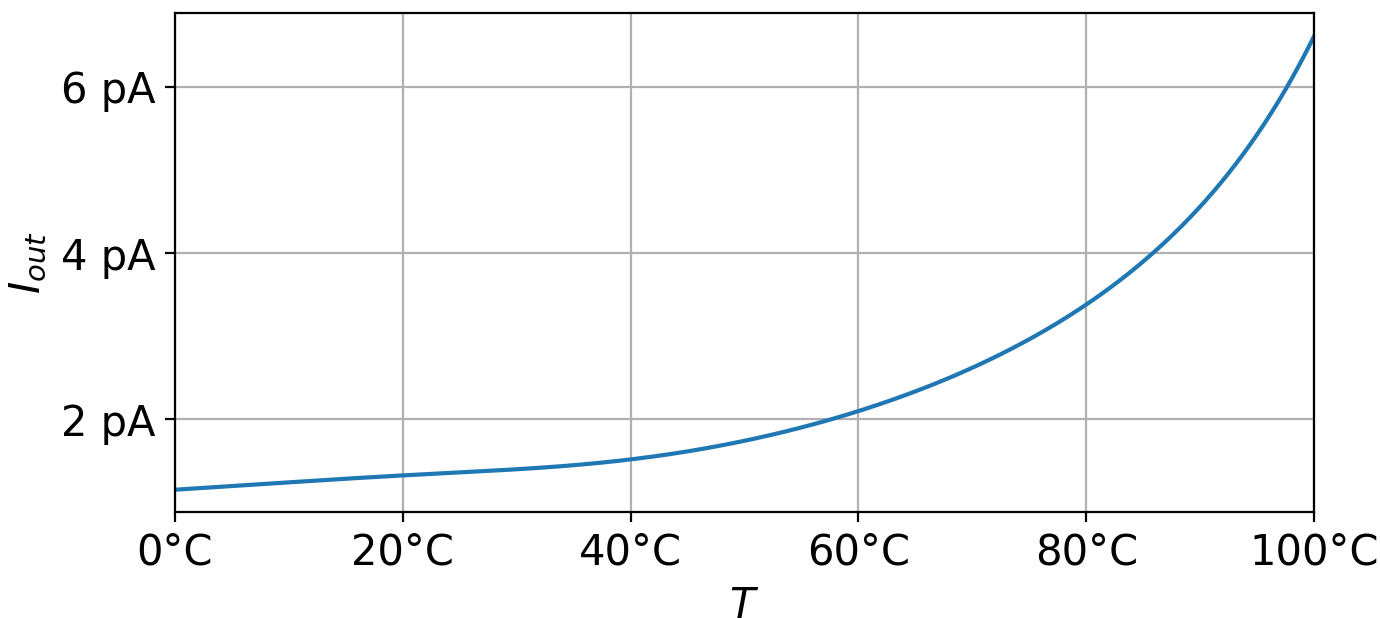
\includegraphics[width=\mysize\linewidth]{Imagens/mirror_temp_sweep.png}
    \centering
    \caption{Gráfico da sensibilidade térmica da fonte completa para $V_{dd}=V_{out}=\sis{1.8}{\volt}$.}
    \label{fig:mirror_temp_sweep}
\end{figure}

\begin{wrapfigure}[9]{r}{0.21\textwidth}
    \centering
    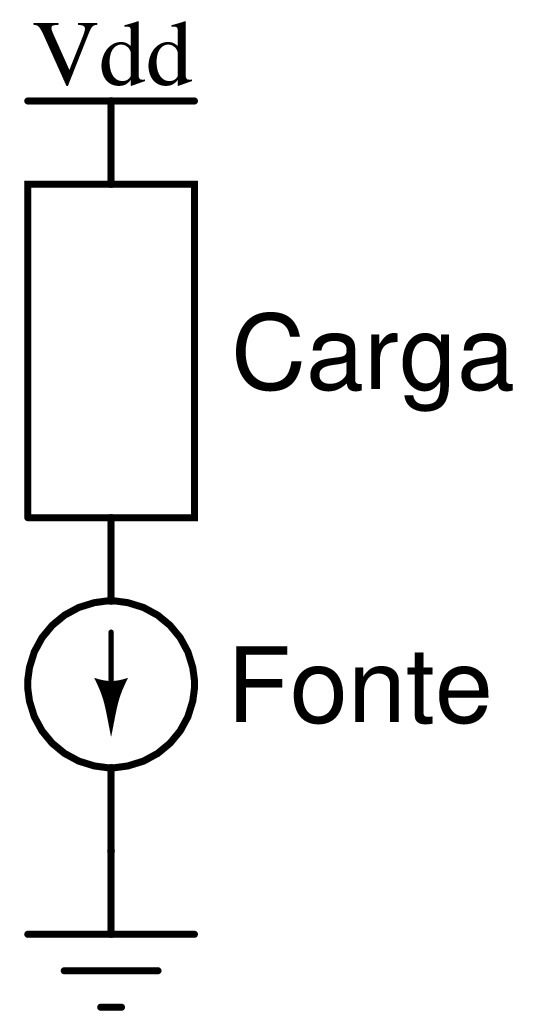
\includegraphics[width=0.13\textwidth]{Imagens/loaded_sbcs.jpg}
    \caption{Fonte de corrente com carga.}
    \label{fig:loaded_sbcs}
\end{wrapfigure}

A fonte de corrente é do tipo \textit{sink}, isto é, a sua carga fica conectada entre a alimentação $V_{dd}$ e a saída da fonte, como pode ser visto na figura \ref{fig:loaded_sbcs}. Até agora, os gráficos de regulação de linha foram traçados partindo do pressuposto de que a tensão de saída é mantida fixa independente das variações na alimentação. O diagrama da figura \ref{fig:loaded_sbcs} nos permite ver que, dependendo da carga, a tensão de saída poderia variar com a alimentação.\endnote{Por exemplo, se assumirmos uma carga puramente resistiva $R_L$, podemos verificar que

\begin{equation}
    \label{eq:vout_vdd}
    V_{out}=V_{dd}-R_LI_{out}
\end{equation}

A tensão de saída depende da alimentação de duas formas. A primeira é o termo linear em \eqref{eq:vout_vdd}. A segunda é através de $I_{out}$ que depende de $V_{dd}$ além de depender também do próprio $V_{out}$.
} Vamos analisar o pior caso o possível, isto é, o caso da carga ser um curto-circuito e $V_{out}=V_{dd}$.

\begin{figure}[htp!]
    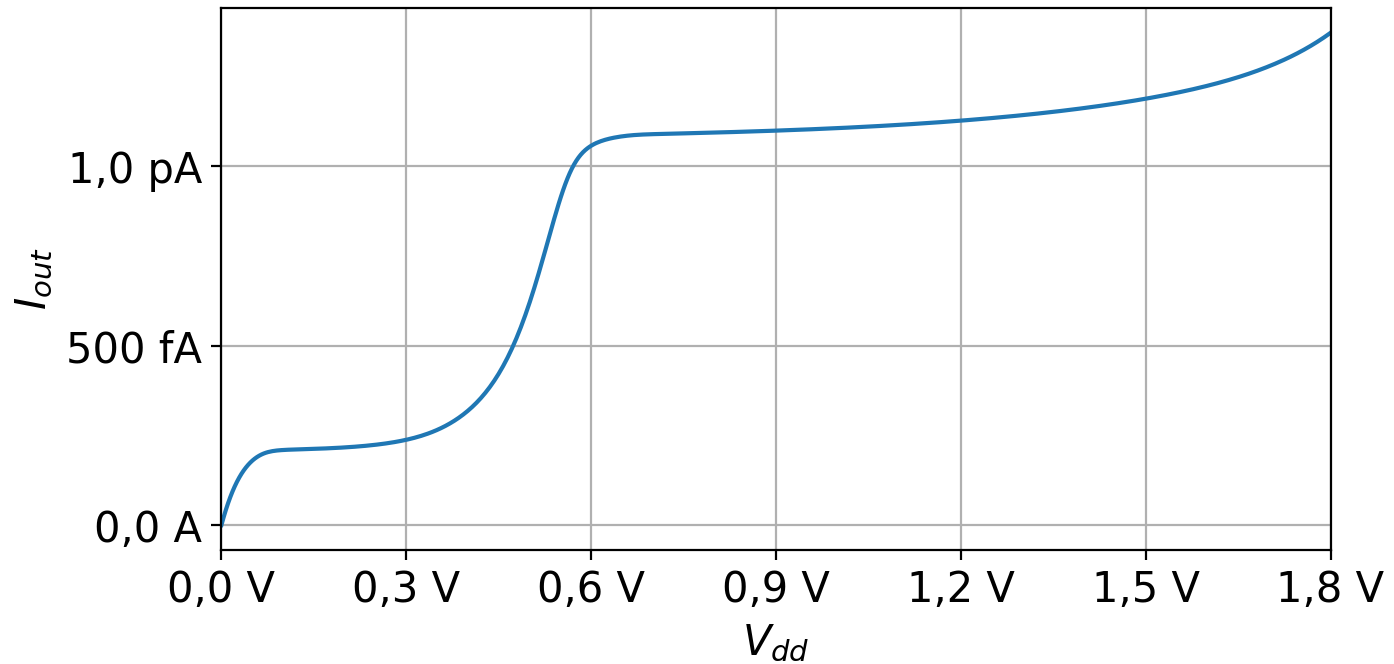
\includegraphics[width=\mysize\linewidth]{Imagens/mirror_vout_equal_vdd.png}
    \centering
    \caption{Gráfico da regulação de linha da fonte de corrente completa para $V_{out}=V_{dd}$.}
    \label{fig:mirror_vout_equal_vdd}
\end{figure}

Podemos ver na figura \ref{fig:mirror_vout_equal_vdd} que a regulação se tornou consideravelmente pior. A sensibilidade média à alimentação na faixa de $\sis{700}{\milli\volt}$ até $\sis{1.8}{\volt}$ foi de $\sis{20.9}{\percent\per\volt}$. A potência total consumida pelo circuito nesta configuração foi $\sis{133.1}{\pico\watt}$.

\chapter{Resultados e Discussão}

Este projeto apresentou especificações bem soltas. A única verdadeira restrição era conseguir uma corrente nas proximidades de $\sis{1}{\pico\ampere}$, um objetivo que foi alcançado. O projeto também tentou alcançar uma boa regulação de linha e baixa sensibilidade térmica, mas nenhum valor máximo foi estipulado \textit{a priori}. Por isso, a avaliação final das sensibilidades foi feita com certo grau de subjetividade. Foi alcançada uma corrente de saída de $\sis{1.371}{\pico\ampere}$ com uma sensibilidade à alimentação que não ultrapassa $\sis{4}{\percent\per\volt}$ e uma sensibilidade térmica de $\sis{1.75}{\percent\per\celsius}$.

Um problema apresentado pelo projeto é a baixa regulação de linha quando a tensão de saída varia junto com a alimentação. Analisamos o pior caso, isto é, quando a carga é um curto-circuito ($V_{out}=V_{dd}$) e medimos uma sensibilidade de $\sis{20.9}{\percent\per\volt}$. Mesmo sem uma especificação numérica para a regulação é difícil aceitar uma sensibilidade tão elevada. Para se remediar tal problema poderia se isolar $V_{out}$ de $V_{dd}$. Isso poderia ser realizado através de um projeto de alguma carga adaptativa que consiga manter a tensão de saída aproximadamente constante.\endnote{Podemos utilizar \eqref{eq:vout_vdd} para obtermos uma relação que uma carga adaptativa $R_L$ perfeita precisaria obedecer. Para isso, vamos derivar ambos os lados de \eqref{eq:vout_vdd} em relação a $V_{dd}$:

\begin{equation}
    \label{eq:vout_deiv_vdd}
    \pd{V_{out}}{V_{dd}}{}=1-\pd{R_L}{V_{dd}}{}\cdot I_{out}-R_L\left(\pd{I_{out}}{V_{dd}}{}+\pd{I_{out}}{V_{out}}{}\cdot\pd{V_{out}}{V_{dd}}{}\right)
\end{equation}

Como queremos que $V_{out}$ e $V_{dd}$ estejam isolados um do outro, vamos substituir $\pd{V_{out}}{V_{dd}}{}=0$ em \eqref{eq:vout_deiv_vdd}, nos resultando em

\begin{equation}
    \label{eq:adaptative_load}
    \pd{R_L}{V_{dd}}{}\cdot I_{out}+R_L\cdot\pd{I_{out}}{V_{dd}}{}=1
\end{equation}

Se \eqref{eq:adaptative_load} é válida para qualquer valor de $V_{dd}$ e $I_{out}$, a isolação seria perfeita de forma incondicional. Se \eqref{eq:adaptative_load} é válida apenas no ponto desejado de operação, a isolação seria apenas local. Caso a tensão de alimentação seja relativamente bem ajustada, tal aproximação local poderia ser considerada aceitável.}





\newpage
\renewcommand{\thechapter}{N}
\printendnotes[custom]
\newpage
\addcontentsline{toc}{chapter}{Referências}
\printbibliography

\end{document}
